\documentclass[10pt,a4paper]{article}

\usepackage{appendix}
\usepackage{graphicx}
\usepackage{parskip}
\usepackage{listings}
\usepackage{caption}
\usepackage{subcaption}
\usepackage{amsmath}
\usepackage{listings}
\usepackage{xcolor}
\usepackage[most]{tcolorbox}

%%%%%%%%%%%%%%%%%%%%%%%%%%%%%%%%%%%%%%%%%%%%%%%%%%%%%%%%%%%%%%%%%%%%%%%%%%%%%%%%%%%%%%%%%%%%%%%%%%%%%%%%%%
\definecolor{codegreen}{rgb}{0,0.6,0}
\definecolor{codegray}{rgb}{0.5,0.5,0.5}
\definecolor{codepurple}{rgb}{0.58,0,0.82}
\definecolor{backcolour}{rgb}{1,1,1}

\lstdefinestyle{mystyle}
{
    backgroundcolor=\color{backcolour},   
    commentstyle=\color{codegreen},
    keywordstyle=\color{magenta},
    numberstyle=\tiny\color{codegray},
    stringstyle=\color{codepurple},
    basicstyle=\ttfamily\footnotesize,
    breakatwhitespace=false,         
    breaklines=true,                 
    captionpos=b,                    
    keepspaces=true,                 
    numbers=left,                    
    numbersep=5pt,                  
    showspaces=false,                
    showstringspaces=false,
    showtabs=false,                  
    tabsize=2
}

\lstset{style=mystyle}
%%%%%%%%%%%%%%%%%%%%%%%%%%%%%%%%%%%%%%%%%%%%%%%%%%%%%%%%%%%%%%%%%%%%%%%%%%%%%%%%%%%%%%%%%%%%%%%%%%%%%%%%%%

\lstset{basicstyle=\ttfamily, breaklines = true, tabsize=2}
\graphicspath{ {./Images/} }
\setlength{\parskip}{1em}
\begin{document}
%%%%%%%%%%%%%%%%%%%%%%%%%%%%%%%%%%%%%%%%%%%%%%%%%%%%%%%%%%%%%%%%%%%%%%%%%%%%%%%%%%%%%%%%%%%%%%%%%%%%%%%%%%

\begin{titlepage}
	\centering
	{\scshape\LARGE Imperial College London \par}
	\vspace{1cm}
    {\scshape\Large Mathematics: Year 2\par}
    \vspace{1.5cm}
	{\huge\bfseries Vectors (Field Theory)\par}
	\vspace{2cm}
	{\Large\ Xin Wang }
	\vfill
	{\large \today\par}
\end{titlepage}

%%%%%%%%%%%%%%%%%%%%%%%%%%%%%%%%%%%%%%%%%%%%%%%%%%%%%%%%%%%%%%%%%%%%%%%%%%%%%%%%%%%%%%%%%%%%%%%%%%%%%%%%%%

\begin{abstract}
    In engineering, many applications uses functions of the space variable $\textbf{r}=x
    \textbf{i}+y \textbf{j} + z \textbf{k}$ as models for quantities in the 3-D space. Being able to
    manipulate and model quantities effectively is a critical skill in any engineering field.
\end{abstract}

%%%%%%%%%%%%%%%%%%%%%%%%%%%%%%%%%%%%%%%%%%%%%%%%%%%%%%%%%%%%%%%%%%%%%%%%%%%%%%%%%%%%%%%%%%%%%%%%%%%%%%%%%%

\tableofcontents
\pagebreak

%%%%%%%%%%%%%%%%%%%%%%%%%%%%%%%%%%%%%%%%%%%%%%%%%%%%%%%%%%%%%%%%%%%%%%%%%%%%%%%%%%%%%%%%%%%%%%%%%%%%%%%%%%
\section{Revision}

Given the vector notation for a 3-D space: $\textbf{a}=a_1 \textbf{i}+a_2 \textbf{j}+a_3 \textbf{k}
\equiv (a_1,a_2,a_3)$, the critical values are as follows:
\begin{enumerate}
    \item Magnitude/Length of vector:
    $$
        |\textbf{a}| = (a_1^2+a_2^2+a_3^2)^{\frac{1}{2}}
    $$

    \item Scalar/Dot product of two vectors $a$ and $b$:
    $$
        \textbf{a}.\textbf{b}=a_1b_1 + a_2b_2 + a_3b_3
    $$

    \item Angle between two vectors $a$ and $b$:
    $$
        \textbf{a}.\textbf{b}=ab\cos(\theta)
    $$
    where $\textbf{a}.\textbf{b}=0$ means it is perpendicular

    \item Vector/Cross product between two vectors $a$ and $b$:
    $$
    \textbf{a}\times \textbf{b} = 
    \begin{vmatrix}
        \textbf{\underline{i}} & \textbf{\underline{j}} & \textbf{\underline{k}} \\
        a_1 & a_2 & a_3 \\
        b_1 & b_2 & b_3
    \end{vmatrix} = [ab\sin(\theta)]\hat{\textbf{n}}
    $$
    where $\hat{\textbf{n}}$ is the unit vector perpendicular to both $a$ and $b$. If $a\times b =
    0$ then both vectors are parallel if neither are null.

    \item Scalar triple product between three vectors $a$, $b$ and $c$:
    $$
    \textbf{a}(\textbf{b} \times \textbf{c}) = 
    \begin{vmatrix}
        a_1 & a_2 & a_3 \\
        b_1 & b_2 & b_3 \\
        c_1 & c_2 & c_3 
    \end{vmatrix}
    $$
    $$
        \textbf{a}(\textbf{b} \times \textbf{c}) \equiv \textbf{b}(\textbf{c} \times \textbf{a}) \equiv \textbf{c}(\textbf{a} \times \textbf{b})
    $$
    where if any two of three vectors are equal then scalar product is zero.

    \item Vector triple product between three vectors $a$, $b$ and $c$:
    $$
        \textbf{a}\times (\textbf{b} \times \textbf{c}) = \textbf{b}(\textbf{a}.\textbf{c}) - \textbf{c}(\textbf{a} . \textbf{b})
    $$
\end{enumerate}

%%%%%%%%%%%%%%%%%%%%%%%%%%%%%%%%%%%%%%%%%%%%%%%%%%%%%%%%%%%%%%%%%%%%%%%%%%%%%%%%%%%%%%%%%%%%%%%%%%%%%%%%%%
\section{Scalar fields}

The essence of field theory is the concept of "action by continuous contact" by which the contact is
provided by a "stress" or "field" induced in the space between the objects by their presence. This
is different form the older view of "action by contact" where it was thought there could only be
action when two objects are touching each other. This older view does not account for other fields
such as gravity and electromagnetism. The modern view developed by James Clerk Maxwell noted that a
force can be exerted on each other \textit{through the presence of an intervening medium or
mechanism existing in the space between objects}. \par

Most applications of vectors in engineering requires dealing with two or more variables. Four
variable functions are commonly encountered e.g. electromagnetism requires three variables for the
3-D space and a variable for time. 

Functions can be represented graphically as fields. In vectors, there are two types of fields
investigated: \textbf{Scalar Fields} and \textbf{Vector Fields}.

\begin{tcolorbox}[breakable,colback=white]
\textbf{Scalar field}: A function that returns a scalar value of some function for every point in
space. 
\\
\\
\textbf{Vector field}: A function that returns a vector value of some function for every point in
space. 
\end{tcolorbox}

%%%%%%%%%%%%%%%%%%%%%%%%%%%%%%%%%%%%%%%%%%%%%%%%%%%%%%%%%%%%%%%%%%%%%%%%%%%%%%%%%%%%%%%%%%%%%%%%%%%%%%%%%%
\subsection{Visualization: Surface plots and Contour plots}

The most common way to visualize is to plot a \textbf{surface plot}. Alternatively a \textbf{contour plot} given by $z=c=constant$ is also common.\par 

\textbf{Example 1}: Given $\phi(x,y)=\frac{1}{12}y^3-y-\frac{1}{4}x^2+\frac{7}{2}$, plot the graph
$z = \phi(x,y)$.

\begin{figure}[h]
\centering
\begin{subfigure}{.5\textwidth}
  \centering
  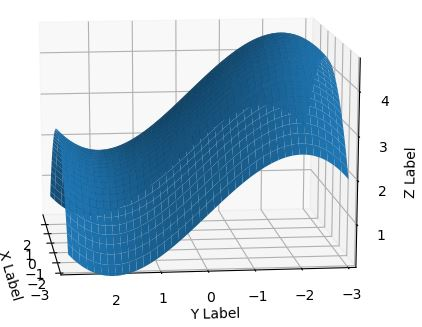
\includegraphics[scale=0.7]{Ex1.JPG}
  \caption{Surface plot}
  \label{fig:sub1}
\end{subfigure}%
\begin{subfigure}{.5\textwidth}
  \centering
  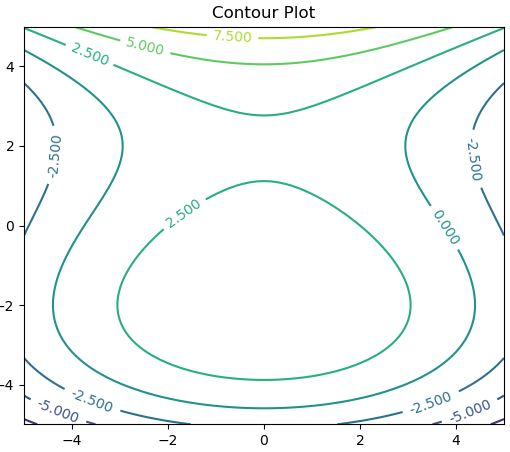
\includegraphics[scale=0.5]{Ex2.JPG}
  \caption{Contour plot}
  \label{fig:sub2}
\end{subfigure}
\label{fig:test}
\end{figure}

Higher dimensions are harder to visualize. One approach is to fix one of the independent variables
e.g. $z$ and then create a contour map for the two remaining dimensions. Each point in a 3D space is
assigned one value ($\phi$) and for each $c$ can be equated $$\phi(x,y,z)=c$$ 

This was seen in previous chapter where each $c$ is a contour line. In a function of three
variables, the contours become \textbf{3-D} contour surfaces by changing the fixed variable. The
contour surfaces become \textbf{level surfaces}.

\begin{tcolorbox}[breakable,colback=white]
    \textbf{Level surfaces} of [$\phi(x,y,z)$] of level $c$: The set of all points in $R^3$ which
    are solutions to:
    $$
        \phi(x,y,z)=c
    $$
\end{tcolorbox}

An important detail to note is that each value of $c$ gives the level surface: $x+y+z=c$ i.e.
\textbf{a series of parallel planes with common normal}. It is due to this detail that scalar fields
commonly represent electric potential since it is derived from energy - it is a scalar field. \par 

\begin{tcolorbox}[breakable,colback=white]
\textbf{Equipotential}: Region in space where every point is at the same potential, usually
referring to the scalar potential.
\end{tcolorbox}
\begin{itemize}
    \item For a function of two variables ($\phi(x,y)=c$), the field gives equipotential \textbf{lines}.
    \item For a function of three variables ($\phi(x,y,z=c)$), the field gives equipotential \textbf{surfaces}.
\end{itemize}

\textbf{Example 2}: Given $\phi(x,y,z)=x^2+y^2+\frac{z^2}{4}$, plot a surface plot showing the
equipotentials. \par 

Equipotentials are given by:
$$
    \phi(x,y,z) = x^2 + y^2 + \frac{z^2}{4} = c
$$
\begin{figure} [h!]
    \centering
    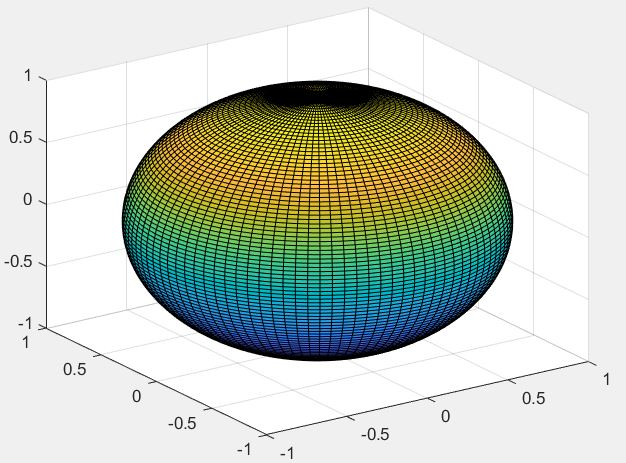
\includegraphics[scale=0.6]{Ellipsoid.JPG}
    \caption{Ellipsoid showing the equipotential surfaces}
\end{figure}

%%%%%%%%%%%%%%%%%%%%%%%%%%%%%%%%%%%%%%%%%%%%%%%%%%%%%%%%%%%%%%%%%%%%%%%%%%%%%%%%%%%%%%%%%%%%%%%%%%%%%%%%%%
\subsection{Scalar fields varying with time}

A scalar field that varies with time has many different ways of being represented. Common ways to
show the change is to overlay two graphs at different times or to plot a surface plot. The methodology
is still the same with time $t$ being a variable.

\textbf{Example 3}: Given the travelling wave in 1D with temporal frequency $F$ and wavelength
$\lambda$:
$$
    f(x,t) = A\cos\left[2\pi \left(Ft - \frac{1}{\lambda}x \right)\right]
$$
Note the common equations: 
\begin{itemize}
    \item Angular Frequency - $\omega = 2\pi F$
    \item Propagation Constant - $k=\frac{2\pi}{\lambda}$
\end{itemize}
$$
    f(x,t)=A\cos(\omega t - kx)
$$

\begin{figure} [h]
\centering
\begin{subfigure}{.5\textwidth}
  \centering
  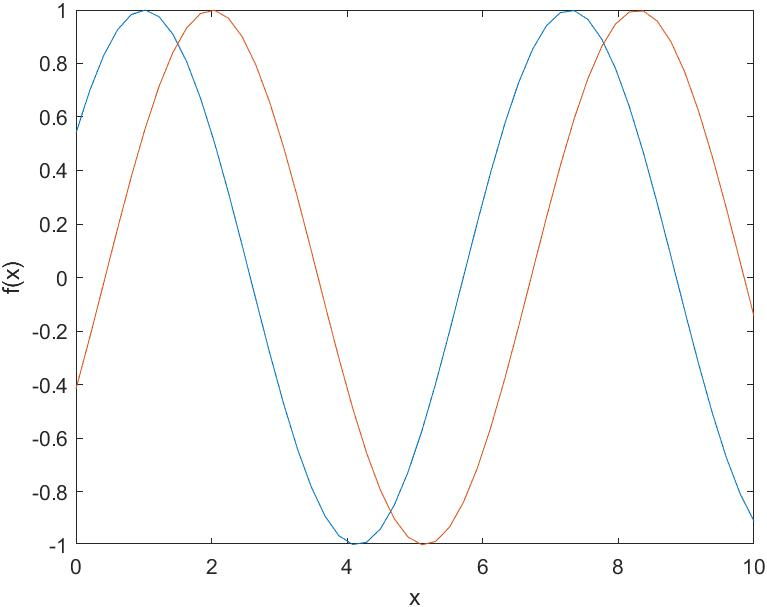
\includegraphics[scale=0.18]{Overlaid.JPG}
  \caption{Same graphs at different time}
  \label{fig:sub1}
\end{subfigure}%
\begin{subfigure}{.5\textwidth}
  \centering
  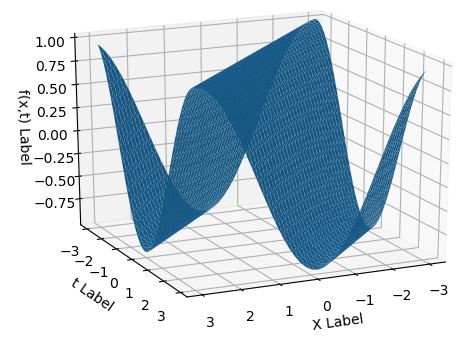
\includegraphics[scale=0.55]{Cos_varying.JPG}
  \caption{Surface plot of graph with time $t$ varying}
  \label{fig:sub2}
\end{subfigure}
\label{fig:test}
\end{figure}

For higher variable functions, the only common approach is to take snapshots of the surface plot
where a variable e.g. $z$ is constant and each snapshot has a different time variable $t$.
\begin{figure} [h!]
    \centering
    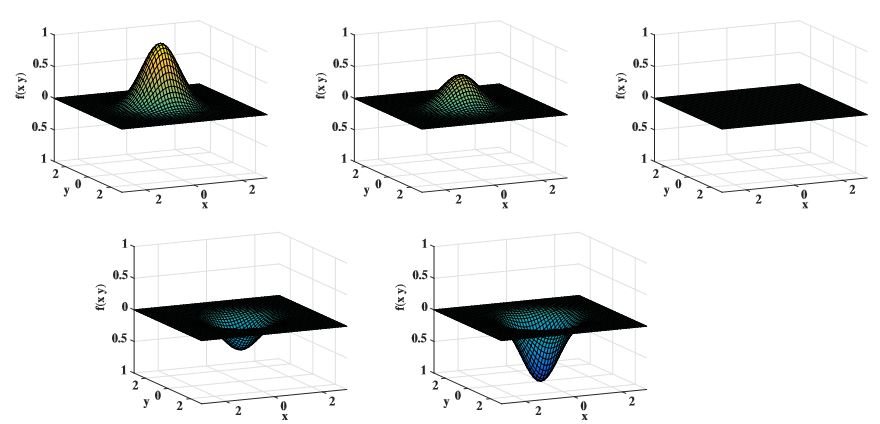
\includegraphics[scale=0.6]{Snapshots.JPG}
    \caption{Snapshots of the same function at different times}
\end{figure}

%%%%%%%%%%%%%%%%%%%%%%%%%%%%%%%%%%%%%%%%%%%%%%%%%%%%%%%%%%%%%%%%%%%%%%%%%%%%%%%%%%%%%%%%%%%%%%%%%%%%%%%%%%
\section{Vector fields}

A \textbf{vector field}: Each point in space is associated with a vector. 
\begin{itemize}
    \item When displaying a vector field, the vectors (arrows) are \textbf{normalized} to prevent
    very large arrows from crowding out smaller vectors.
    \item Vector field vectors change over time i.e. seen in wind.
    \item Vector fields can be 3-D or 2-D.
\end{itemize}

It is useful to imagine a vector field with \textbf{fluid flow} to help with understanding the
theory.

A vector field has components in terms of the \textbf{three unit vectors} 
$(\textbf{\underline{i}},\textbf{\underline{j}},\textbf{\underline{k}})$.
$$
    \textbf{\underline{B}} = \textbf{\underline{i}}B_1(x,y,z,t)+\textbf{\underline{j}}B_2(x,y,z,t)+\textbf{\underline{k}}B_3(x,y,z,t)
$$
where $B_n$ are all\textbf{scalar fields}. \par 

%%%%%%%%%%%%%%%%%%%%%%%%%%%%%%%%%%%%%%%%%%%%%%%%%%%%%%%%%%%%%%%%%%%%%%%%%%%%%%%%%%%%%%%%%%%%%%%%%%%%%%%%%%
\subsection{Visualization of vector fields}

The most common are \textbf{field plots} where an arrow represents the direction/magnitude of the
field - the vector at the point. 

When plotting field plots:
\begin{enumerate}
    \item Plot direction with vectors on the axes.
    \item If necessary, plot directions of vectors on lines $y=\pm x$.
    \item Spot the pattern and complete.
\end{enumerate}

\textbf{Example 1}: Given
$\textbf{\underline{F}}(x,y)=y\textbf{\underline{i}}-x\textbf{\underline{j}}$

\begin{figure} [h!]
    \centering
    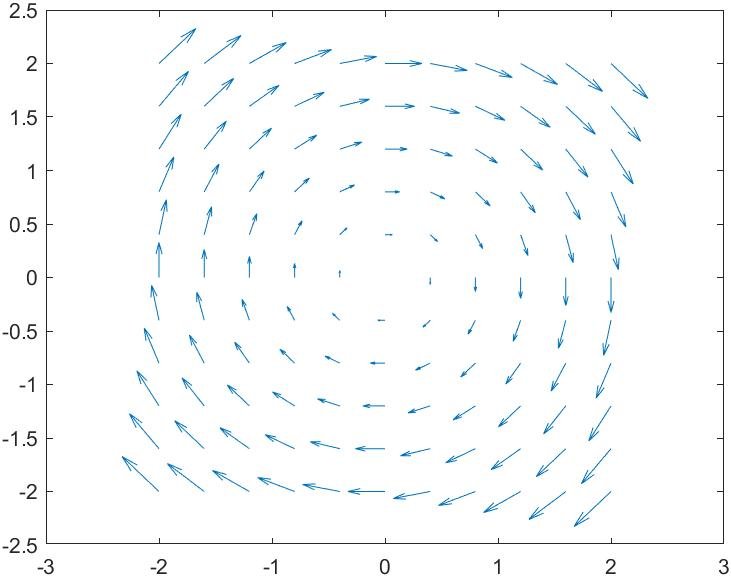
\includegraphics[scale=0.25]{Vector field.JPG}
    \caption{Field plot}
\end{figure}

\begin{tcolorbox}[breakable,colback=white]
\textbf{Field lines}: Graphical aid for visualizing vector fields. Consists of a directed line which
is parallel to the vector field. Note it does not give the direction of the flow.
\end{tcolorbox}

On vector fields, \textbf{field lines} can be drawn by following the gradient relationship:

\begin{tcolorbox}[breakable,colback=white]
Given a 2-D field $\textbf{\underline{F}}=F_x \textbf{\underline{i}} + F_y \textbf{\underline{j}}$ and
the field lines $y=y(x)$, the relationship between the vector field and field lines are:
$$
    \frac{dy}{dx}=\frac{F_y}{F_x}
$$
\end{tcolorbox}

Following \textbf{Example 1}, the relationship causing the field plot is defined: 
$$
    \frac{dy}{dx} = - \frac{x}{y} \rightarrow y\text{ }dy = -x\text{ }dx
$$

Through integration, the field line equation is $x^2 + y^2 = c$ which is evident as a circle seen in Figure 5.

\textbf{Example 2}: Given a line of electric charge parallel to the $z$-axis, the electric field
$\textbf{\underline{E}}$ is radial, confirming with electric charge theory from physics.
$$
    \textbf{\underline{E}}=\frac{q}{2\pi \epsilon_0 r}\hat{\textbf{\underline{r}}}
$$
where:
\begin{itemize}
    \item $r=\sqrt{x^2 + y^2}$ - Distance from the origin
    \item $q$ - Charge per unit Length
    \item $\epsilon_0$ - Permittivity of free space
    \item $\hat{\textbf{\underline{r}}}$ - Unit vector in radial direction
\end{itemize}

\begin{figure} [h!]
    \centering
    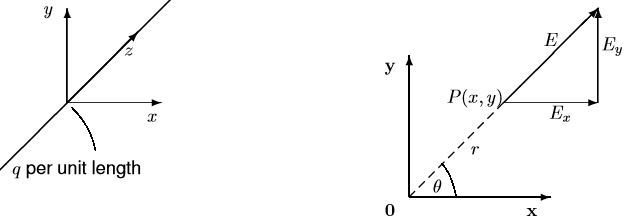
\includegraphics[scale=0.7]{Charge.JPG}
    \caption{Graphical representation of line of charge on the $z$-axis}
\end{figure}

This allows an equation to be formed in terms of Cartesian components:
\begin{align*}
    \textbf{\underline{E}} &= E_x \textbf{\underline{i}} + E_y \textbf{\underline{j}} \\
    &= \frac{k}{r}\cos(\theta)\textbf{\underline{i}} + \frac{k}{r}\sin(\theta)\textbf{\underline{j}}
\end{align*}
where $k=\frac{q}{2\pi \epsilon_0}$ \par 

Given that $\cos(\theta)=\frac{x}{r}$ and $\sin(\theta)=\frac{y}{r})$, the equation simplifies to:
$$
    \textbf{\underline{E}} = \frac{kx}{x^2 + y^2}\textbf{\underline{i}} + \frac{ky}{x^2+y^2}\textbf{\underline{j}}
$$
\begin{figure} [h!]
    \centering
    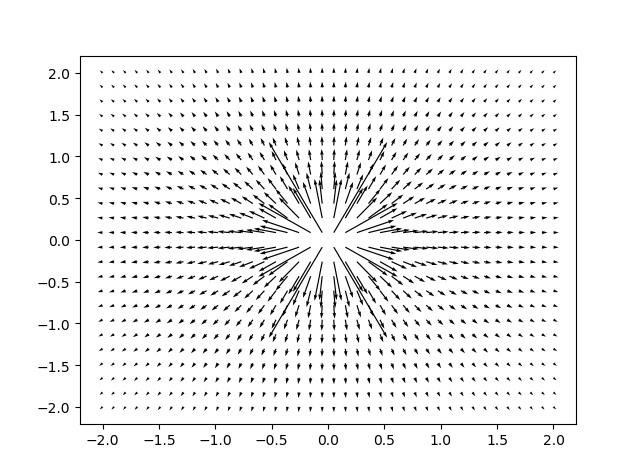
\includegraphics[scale=0.3]{Charge_field.JPG}
    \caption{Vector field of electric charge}
\end{figure}

By shifting the charge from the origin to $(-d,0)$, the equation becomes $r^2=(x+d)^2 + y^2$:
$$
    \textbf{\underline{E}} = \frac{k(x+d)}{(x+d)^2+y^2} \textbf{\underline{i}} + \frac{ky}{(x+d)^2 + y^2} \textbf{\underline{j}}
$$
\begin{figure} [h!]
    \centering
    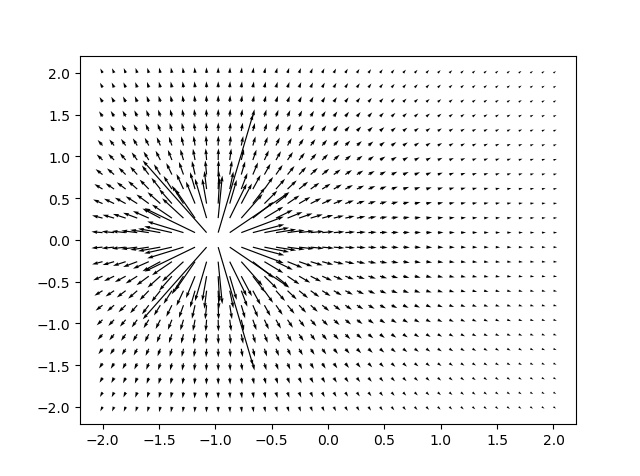
\includegraphics[scale=0.3]{Charge_field2.JPEG}
    \caption{Shifted vector field of electric charge}
\end{figure}

By taking two line charges at $(\pm d,0)$ with strength $\mp q$ per unit length, superposition can be
used to draw the field where the total electric field is the sum of individual fields
$\textbf{\underline{E}} = \textbf{\underline{E}}_1 + \textbf{\underline{E}}_2$:
\begin{align*}
    \textbf{\underline{E}}_1=\frac{q}{2\pi \epsilon_0 r_1}\hat{\textbf{\underline{r}}}_1 = \frac{k}{r_1}\hat{\textbf{\underline{r}}}_1 \quad \text{and} \quad \textbf{\underline{E}}_2=-\frac{q}{2\pi \epsilon_0 r_2}\hat{\textbf{\underline{r}}}_2=-\frac{k}{r_2}\hat{\textbf{\underline{r}}}_2
\end{align*}
\begin{figure} [h!]
    \centering
    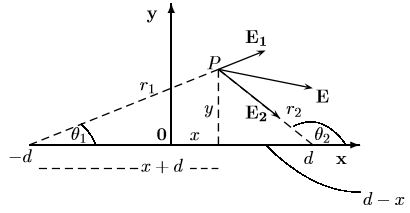
\includegraphics[scale=0.8]{Superposition.JPG}
    \caption{Superposition of two vectors resulting in a resultant vector}
\end{figure}

Simplifying:
\begin{align*}
    E_x&=\frac{k}{r_1}\frac{x+d}{r_1}-\frac{k}{r_2}\frac{x-d}{r_2} = \left(\frac{x+d}{(x+d)^2+y^2 - \frac{x-d}{(x-d)^2+y^2}}\right) \\
    E_y&=\frac{k}{r_1}\frac{y}{r_1}-\frac{k}{r_2}\frac{y}{r_2} = \left(\frac{y}{(x+d)^2+y^2 - \frac{y}{(x-d)^2+y^2}}\right)
\end{align*}

Resulting in the following vector field:
\begin{figure} [h!]
    \centering
    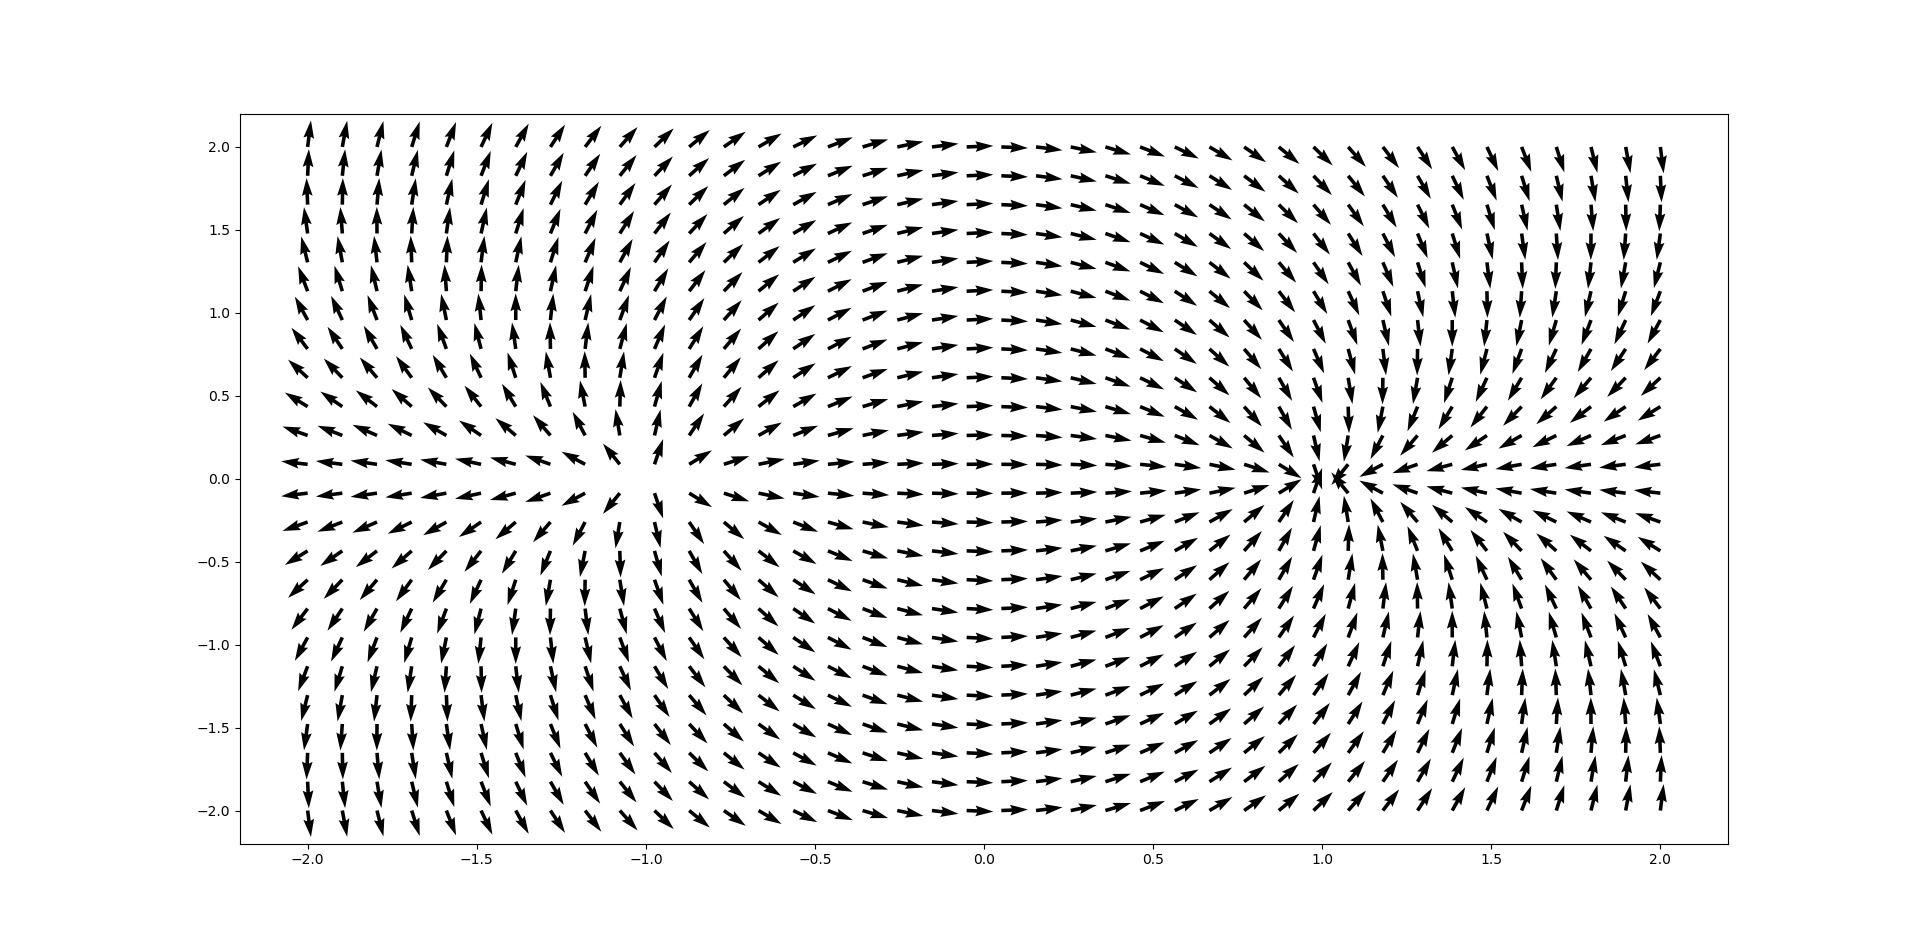
\includegraphics[scale=0.2]{Superposition_field.jpeg}
    \caption{Graphical representation of the superimposed vector field}
\end{figure}

%%%%%%%%%%%%%%%%%%%%%%%%%%%%%%%%%%%%%%%%%%%%%%%%%%%%%%%%%%%%%%%%%%%%%%%%%%%%%%%%%%%%%%%%%%%%%%%%%%%%%%%%%%
\section{Vector operators: Grad, Div and Curl}
%%%%%%%%%%%%%%%%%%%%%%%%%%%%%%%%%%%%%%%%%%%%%%%%%%%%%%%%%%%%%%%%%%%%%%%%%%%%%%%%%%%%%%%%%%%%%%%%%%%%%%%%%%
\subsection{Gradient Operator $(\nabla)$}

In a scalar field $(\phi)=\phi(x,y,z)$, \textbf{how quickly the scalar field varies} in the $x$, $y$ and $z$
direction is defined as:
$$
    \frac{\partial \phi}{\partial x} \quad \text{ or } \quad \frac{\partial \phi}{\partial y} \quad \text{ or } \quad \frac{\partial \phi}{\partial z}
$$
\textbf{Note: $\phi$ is a scalar field but $\nabla\phi$ is a vector field.}
\begin{tcolorbox}[breakable,colback=white]
    \textbf{Gradient}: How quickly the potential varies at any point:
    $$
        grad\text{ }\phi=\nabla\phi=\textbf{\underline{i}}\frac{\partial \phi}{\partial x} + \textbf{\underline{j}}\frac{\partial \phi}{\partial y} + \textbf{\underline{k}}\frac{\partial \phi}{\partial z}
    $$
\end{tcolorbox}

%%%%%%%%%%%%%%%%%%%%%%%%%%%%%%%%%%%%%%%%%%%%%%%%%%%%%%%%%%%%%%%%%%%%%%%%%%%%%%%%%%%%%%%%%%%%%%%%%%%%%%%%%%
\subsubsection{Directional derivatives}

When considering the rate of change of scalar $\phi$ \textbf{in a particular direction}, denote the
direction by unit vector $\hat{\textbf{m}}$ i.e. if direction
$\hat{\textbf{m}}=\textbf{\underline{i}}$ then $\hat{\textbf{m}}=\frac{\partial \phi}{\partial x}$.

Thus following the notation, the following points must be noted:
\begin{itemize}
    \item Component of a vector \textbf{in the direction of a unit vector} is given by the
    \textbf{scalar product} i.e. $\nabla \phi . \hat{\textbf{m}}$.
    \item Directional derivative of $\phi$ in the direction of unit vector $\hat{\textbf{m}}$ is
    \textbf{equal to} the rate of change of $\phi$ in direction of unit vector $\hat{\textbf{m}}$:
    $$
    \nabla\phi.\hat{\textbf{m}} = \frac{\partial \phi}{\partial \hat{\textbf{m}}} 
    $$
\end{itemize}

\textbf{Note}: $\frac{\partial \phi}{\partial \hat{\textbf{m}}}$ is a scalar

%%%%%%%%%%%%%%%%%%%%%%%%%%%%%%%%%%%%%%%%%%%%%%%%%%%%%%%%%%%%%%%%%%%%%%%%%%%%%%%%%%%%%%%%%%%%%%%%%%%%%%%%%%
\subsubsection{Gradient of a scalar field}

The gradient of a scalar field can represent physical aspects in a scalar field like the
electric potential ($\phi$) where the curves representing contour lines where the
potential is constant.

\begin{figure} [h!]
    \centering
    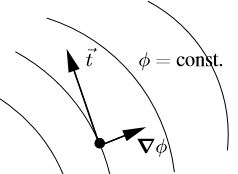
\includegraphics[scale=0.75]{Electric_field.JPG}
\end{figure}

Since a contour line represents where gradient does not change, the potential along the contour line
does not change. This is defined by setting direction vector $\hat{\textbf{m}}$ as along the contour
line:
$$
    \nabla\phi.\hat{\textbf{m}}=\frac{\partial \phi}{\partial \hat{\textbf{m}}}= 0
$$
or where $\overrightarrow{t}$ is tangent to a level surface i.e. contour line:
$$
    \nabla\phi.\overrightarrow{t} = 0
$$
It means that the vector field $(\nabla\phi)$ is \textbf{always} perpendicular to the tangent or
contour line thus it is perpendicular to the plane $\phi(x,y,z)$. This means that the vector
representing the gradient change in the field $\phi$ - $\nabla\phi$ - always points to the direction where $\phi$ varies the most rapidly:
\begin{align*}
    \nabla\phi &= \left(\hat{\textbf{i}}\frac{\partial \phi}{\partial x}+\hat{\textbf{j}}\frac{\partial \phi}{\partial y} + \hat{\textbf{k}}\frac{\partial \phi}{\partial z}\right) \\
    &= \frac{\partial\phi}{\partial\overrightarrow{n}}\hat{\textbf{n}}
\end{align*}
where the normal vector $(\hat{\textbf{n}})$ is in the direction of the greatest increase of $\phi(\overrightarrow{r})$:
$$
    \hat{\textbf{n}} = \frac{\nabla \phi}{|\nabla\phi|}
$$
where $\frac{\partial \phi}{\partial \overrightarrow{n}}$ is the normal derivative to surface

\pagebreak

\textbf{Example 1}: Examine the 2-D scalar field $\phi(x,y)=e^{-x^2-y^2}$. Note that $\phi=C$
implies $x^2+y^2 = constant$. 
\begin{figure*} [h]
    \centering
    \begin{subfigure}{.5\textwidth}
      \centering
      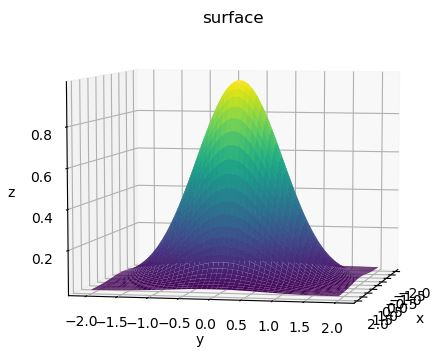
\includegraphics[scale=0.35]{exp_scalar.JPEG}
      \caption{Surface plot}
      \label{fig:sub1}
    \end{subfigure}%
    \begin{subfigure}{.5\textwidth}
      \centering
      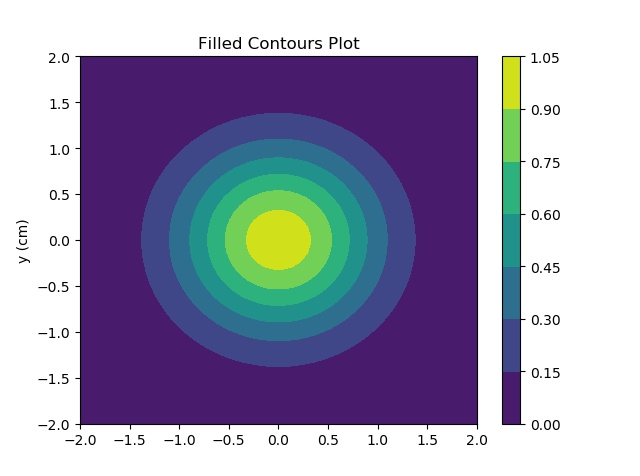
\includegraphics[scale=0.35]{exp_contour.jpeg}
      \caption{Contour plot}
      \label{fig:sub2}
    \end{subfigure}
    \caption*{}
    \label{fig:test}
\end{figure*}

Obtain the $\nabla\phi$:
$$
    \nabla \phi = \left(-2xe^{-x^2-y^2}\right)\textbf{\underline{i}}-\left(2ye^{-x^2-y^2}\right)\textbf{\underline{j}}
$$
\begin{figure*} [h]
    \centering
    \begin{subfigure}{.5\textwidth}
      \centering
      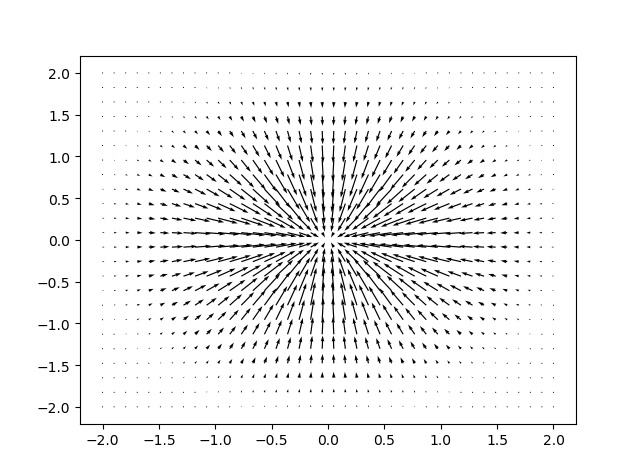
\includegraphics[scale=0.35]{exp_quiver.jpeg}
      \caption{Gradient field}
      \label{fig:sub1}
    \end{subfigure}%
    \begin{subfigure}{.5\textwidth}
      \centering
      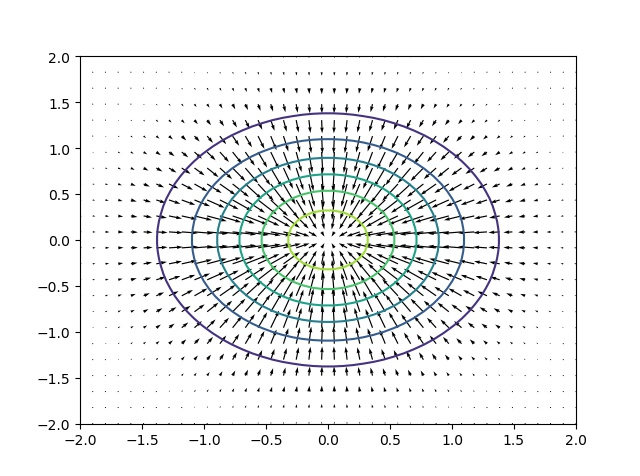
\includegraphics[scale=0.35]{exp_contour_quiver.jpeg}
      \caption{Equipotential lines with gradient field}
      \label{fig:sub2}
    \end{subfigure}
    \label{fig:test}
\end{figure*}

\textbf{Note}:
\begin{itemize}
    \item The vectors are pointing toward the center - the direction of greatest change in gradient ($\phi$)
    \item Equipotential lines and gradient field lines are clearly perpendicular
\end{itemize} 

%%%%%%%%%%%%%%%%%%%%%%%%%%%%%%%%%%%%%%%%%%%%%%%%%%%%%%%%%%%%%%%%%%%%%%%%%%%%%%%%%%%%%%%%%%%%%%%%%%%%%%%%%%
\subsection{Derivatives of Vector Point Function}

When considering the vector field $\phi$, there are two ways of combining the vector operator
$\nabla$ with $\phi$: $\nabla \textbf{ . }\phi$ and $\nabla \times \phi$. Both derivatives have
physical meanings.

\textbf{Note that $grad\text{ }\phi = \nabla\phi$ are two different concepts.} 

Vector algebra has two types of products: \textbf{Scalar} and \textbf{Vector}. 
\begin{itemize}
    \item Scalar products: 
    \begin{itemize}
        \item Results in a scalar - a number.
        \item Used to define work and energy relationships.
    \end{itemize}
    \item Vector products:
    \begin{itemize}
        \item Results in another vector.
        \item Mainly used to derive other vector quantities e.g. vector "torque" defined as vector
        product of an applied force (vector) and distance from pivot (number).
    \end{itemize}
\end{itemize}

The relation between these two are often given in a vector field example with fluid flow: At every point
in the fluid flow, there are two aspects:
\begin{itemize}
    \item Scalar product - The rate at which the field is flowing away from that point
    \item Vector product - The amount of spin possessed by the particle of fluid at that point
\end{itemize}

%%%%%%%%%%%%%%%%%%%%%%%%%%%%%%%%%%%%%%%%%%%%%%%%%%%%%%%%%%%%%%%%%%%%%%%%%%%%%%%%%%%%%%%%%%%%%%%%%%%%%%%%%%
\subsubsection{Divergence of a vector field (\textbf{div} $B$)}

\begin{tcolorbox}[breakable,colback=white]
    \textbf{div}($B$): A measure of the compression/expansion of a vector field in cube (sphere in the case of liquid).
    \begin{itemize}
        \item div $B = 0$: Vector field $B$ is incompressible.
        \item div $B > 0$: Vector field $B$ is expanding.
        \item div $B < 0$: Vector field $B$ is compressing.
    \end{itemize}
\end{tcolorbox}

Given vector field:
$$
    B = \textbf{\underline{i}}[B_1(x,y,z,t)]+\textbf{\underline{j}}[B_2(x,y,z,t)]+\textbf{\underline{k}}[B_3(x,y,z,t)]
$$

The scalar (dot) product:
\begin{align*}
    \textbf{div } \textbf{B} &= \nabla \textbf{ . B} \\
    &= \left(\textbf{\underline{i}}\frac{\partial}{\partial x}+\textbf{\underline{j}}\frac{\partial}{\partial y}+ \textbf{\underline{k}}\frac{\partial}{\partial z}\right)\textbf{ . }\left(\textbf{\underline{i}}B_1+\textbf{\underline{j}}B_2+\textbf{\underline{k}}B_3\right)
\end{align*}

\begin{tcolorbox}[breakable,colback=white]
    Remember that $\textbf{\underline{i}}.\textbf{\underline{i}} =
    \textbf{\underline{j}}.\textbf{\underline{j}}=\textbf{\underline{k}}.\textbf{\underline{k}}=1$ and
    $\textbf{\underline{i}}.\textbf{\underline{j}}=\textbf{\underline{i}}.\textbf{\underline{k}}=\textbf{\underline{k}}.\textbf{\underline{j}}=0$
    thus simplifies to:
    \begin{align*}
        \textbf{div } \textbf{B} = \nabla \textbf{ . }B = \frac{\partial B_1}{\partial x} + \frac{\partial B_2}{\partial y} + \frac{\partial B_3}{\partial z}
    \end{align*}
\end{tcolorbox}

\textbf{Note}: 
\begin{itemize}
    \item div $B$ is a scalar field since \textbf{\textit{div}} is formed through dot product.
    \item $B.\nabla \neq \nabla.B$
\end{itemize}

\textbf{Example 1}: Show that $(F.\nabla)r=F$ for any vector field $F$ where $r=(x,y,z)$.

For any vector $F$: 
\begin{align*}
    (F.\nabla)r &= \left(F_1 \frac{\partial}{\partial x} + F_2\frac{\partial}{\partial y} + F_3\frac{\partial}{\partial z}\right)\left(\hat{\textbf{i}}[x]+\hat{\textbf{j}}[y]+\hat{\textbf{k}}[z]\right) \\
    &= \hat{\textbf{i}}F_1 + \hat{\textbf{j}}F_2 + \hat{\textbf{k}}F_3 \\
    &= F
\end{align*}

\textbf{Example 2}: Consider vector field that is the radial vector in 3-D:
$$
    \overrightarrow{F} = x\hat{\textbf{i}}+y\hat{\textbf{j}}+z\hat{\textbf{k}}
$$
Finding the divergence:
\begin{align*}
    \nabla.\overrightarrow{F} &= \frac{\partial x}{\partial x} + \frac{\partial y}{\partial y} + \frac{\partial z}{\partial z} \\
    &= 1 + 1 + 1 \\
    &= 3
\end{align*}
This shows that the divergence is pointing outward (div $B > 0$).
\begin{figure} [h!]
    \centering
    \begin{subfigure}{.5\textwidth}
      \centering
      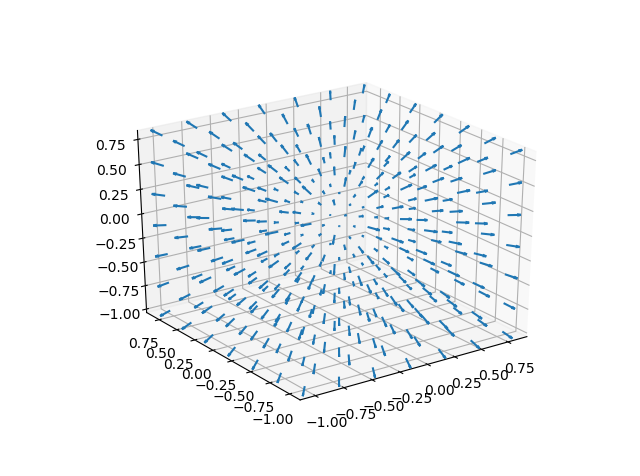
\includegraphics[scale=0.3]{Radial_out.png}
      \caption{Cube showing the circular flow (no flow in the center)}
      \label{fig:sub1}
    \end{subfigure}%
    \begin{subfigure}{.5\textwidth}
      \centering
      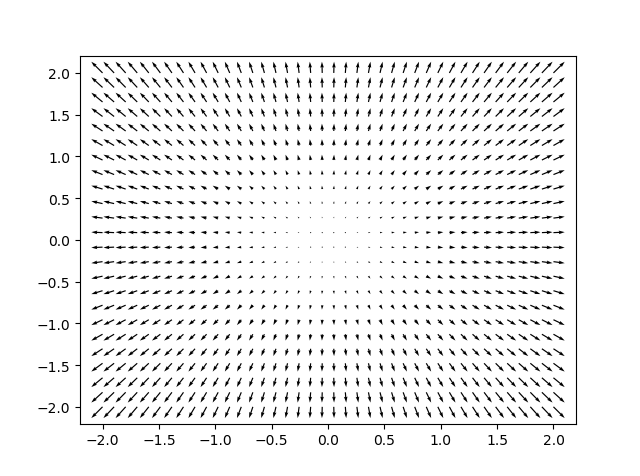
\includegraphics[scale=0.3]{2D_out.png}
      \caption{Arrows pointing into the center}
      \label{fig:sub2}
    \end{subfigure}
    \caption*{}
    \label{fig:test}
\end{figure}

\pagebreak

\textbf{Example 3}: Consider vector field that is the radial vector in 3-D:
$$
    \overrightarrow{F} = -(x\hat{\textbf{i}}+y\hat{\textbf{j}}+z\hat{\textbf{k}})
$$
Finding the divergence:
\begin{align*}
    \nabla.\overrightarrow{F} &= \frac{\partial -x}{\partial x} + \frac{\partial -y}{\partial y} + \frac{\partial -z}{\partial z} \\
    &= -1 - 1 - 1 \\
    &= -3
\end{align*}
This shows that the divergence is pointing inward (div $B < 0$).
\begin{figure} [h]
    \centering
    \begin{subfigure}{.5\textwidth}
      \centering
      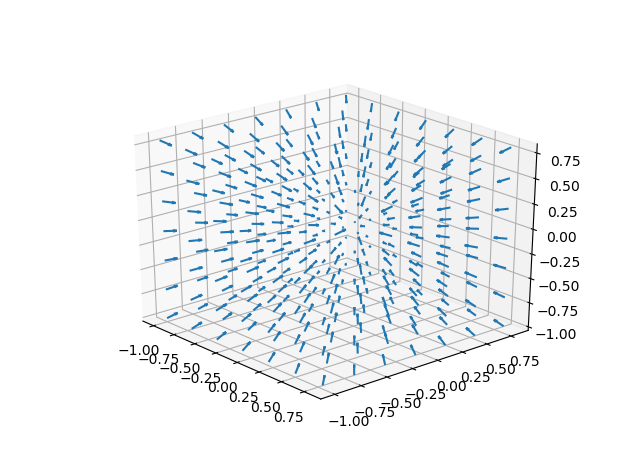
\includegraphics[scale=0.3]{Radial_in.png}
      \caption{Cube showing the circular flow (no flow in the center)}
      \label{fig:sub1}
    \end{subfigure}%
    \begin{subfigure}{.5\textwidth}
      \centering
      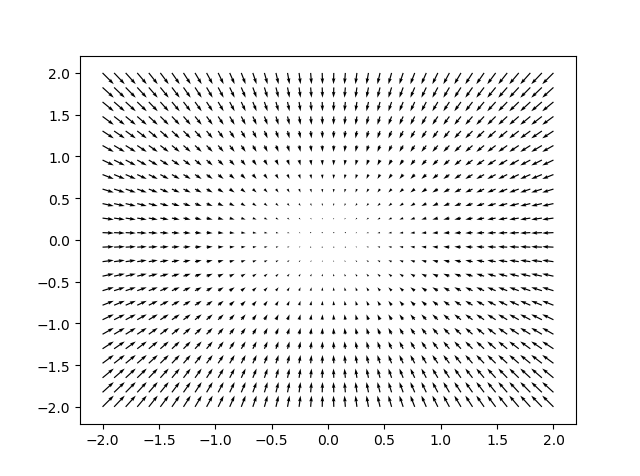
\includegraphics[scale=0.3]{2D_in.png}
      \caption{Arrows pointing into the center}
      \label{fig:sub2}
    \end{subfigure}
    \caption*{}
    \label{fig:test}
\end{figure}

\pagebreak
\textbf{Example 4}: Consider vector field that is the radial vector in 3-D:
$$
    \overrightarrow{F} = y\hat{\textbf{i}}-x\hat{\textbf{j}}+\hat{\textbf{k}})
$$
Finding the divergence:
\begin{align*}
    \nabla.\overrightarrow{F} &= \frac{\partial y}{\partial x} + \frac{\partial -x}{\partial y} + \frac{\partial (1)}{\partial z} \\
    &= 0 - 0 + 0 \\
    &= 0
\end{align*}
This shows that there is no flow into or out of the center (div $B = 0$).
\begin{figure}[h]
\centering
\begin{subfigure}{.5\textwidth}
  \centering
  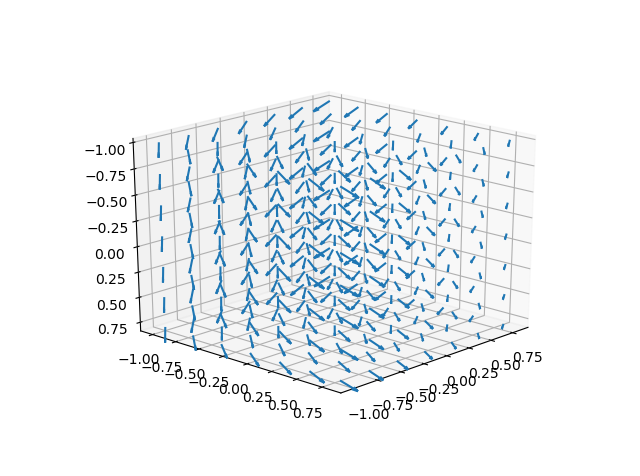
\includegraphics[scale=0.3]{Radial_none.png}
  \caption{Cube showing the circular flow (no flow in the center)}
  \label{fig:sub1}
\end{subfigure}%
\begin{subfigure}{.5\textwidth}
  \centering
  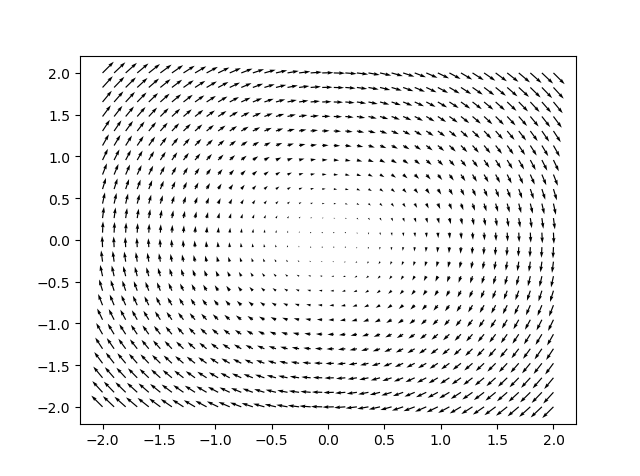
\includegraphics[scale=0.3]{2D_none.png}
  \caption{No flow into or out of the center}
  \label{fig:sub2}
\end{subfigure}
\caption*{}
\label{fig:test}
\end{figure}

The three examples show the three possible cases for divergence of a vector field.
\begin{figure} [h!]
    \centering
    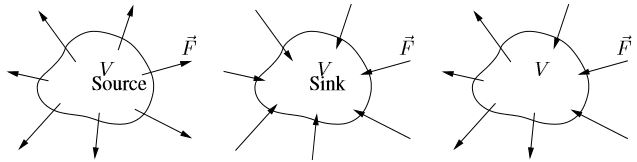
\includegraphics[scale=0.7]{Three.JPG}
    \caption{Three types of possible divergence}
\end{figure}
\begin{enumerate}
    \item div $B > 0$: Vector field $B$ is expanding - V is a source.
    \item div $B < 0$: Vector field $B$ is compressing - V is a sink.
    \item div $B = 0$: Vector field $B$ is incompressible - no net outflow or inflow into region V.
\end{enumerate}

%%%%%%%%%%%%%%%%%%%%%%%%%%%%%%%%%%%%%%%%%%%%%%%%%%%%%%%%%%%%%%%%%%%%%%%%%%%%%%%%%%%%%%%%%%%%%%%%%%%%%%%%%%
\subsubsection{Derivatives of Vector Point Function: Curl of a vector field ($B$)}

The second type of vector multiplication is the Cross Product. 

\begin{tcolorbox}[breakable,colback=white]
    \textbf{Curl}: A vector operator that describes the infinitesimal rotation of a vector field. The attributes of this vector characterize the rotation at that point.
    $$
        \textbf{curl }B = \nabla \times B = \begin{bmatrix}
            \textbf{\underline{i}} & \textbf{\underline{j}} & \textbf{\underline{k}} \\
            \frac{\partial}{\partial x} & \frac{\partial}{\partial y} & \frac{\partial}{\partial z} \\
            B_1 & B_2 & B_3
        \end{bmatrix}
    $$
\end{tcolorbox}

From observations of corks within water, there is rotational motion involved in fluid flow
caused by the fluid particles.

The measure of rotation - curl - is thus a \textbf{vector quantity}. \textbf{A vector field that has a curl cannot diverge and a vector field having divergence cannot curl}.   

\textbf{Example 1}: Straight line vector from origin to a point $(x,y,z)$ denoted
$\textbf{r}=\underline{\textbf{i}}x + \underline{\textbf{j}}y+\underline{\textbf{k}}z$. Find the
curl.
\begin{align*}
    \textbf{curl }\textbf{r} &= \nabla \times \textbf{r} \\
    &= 
    \begin{bmatrix}
        \textbf{\underline{i}} & \textbf{\underline{j}} & \textbf{\underline{k}} \\
        \frac{\partial}{\partial x} & \frac{\partial}{\partial y} & \frac{\partial}{\partial z} \\
        B_1 & B_2 & B_3
    \end{bmatrix} \\
    &= \textbf{\underline{i}}\left[\frac{\partial B_3}{\partial y}-\frac{\partial B_2}{\partial z}\right] - \textbf{\underline{j}}\left[\frac{\partial B_3}{\partial x}-\frac{\partial B_1}{\partial z}\right] + \textbf{\underline{k}}\left[\frac{\partial B_2}{\partial x}-\frac{\partial B_1}{\partial y}\right] \\
    &= 0
\end{align*}

\textbf{Example 2}: Find the curl of vector $\textbf{v}=(2x-y^2,3z+x^2,4y-z^2)$ at point $(1,2,3)$.
\
Assign: $B_1 = 2x-y^2$, $B_2=3z+x^2$ and $B_3=4y-z^2$
\begin{equation*}
    \begin{aligned}
        \textbf{curl }\textbf{v} &= 
        \begin{bmatrix}
            \textbf{\underline{i}} & \textbf{\underline{j}} & \textbf{\underline{k}} \\
            \frac{\partial}{\partial x} & \frac{\partial}{\partial y} & \frac{\partial}{\partial z} \\
            2x-y^2 & 3z+x^2 & 4y-z^2
        \end{bmatrix} \\
        &= \textbf{\underline{i}}\left[\frac{\partial B_3}{\partial y}-\frac{\partial B_2}{\partial z}\right] - \textbf{\underline{j}}\left[\frac{\partial B_3}{\partial x}-\frac{\partial B_1}{\partial z}\right] + \textbf{\underline{k}}\left[\frac{\partial B_2}{\partial x}-\frac{\partial B_1}{\partial y}\right] \\
        &= \textbf{\underline{i}}\left[\frac{\partial}{\partial y}(4y-z^2)-\frac{\partial}{\partial z}(3z+x^2)\right] - \textbf{\underline{j}}\left[\frac{\partial}{\partial x}(4y-z^2)-\frac{\partial}{\partial z}(2x-y^2)\right]\\ &+ \textbf{\underline{k}}\left[\frac{\partial}{\partial x}(3z+x^2)-\frac{\partial}{\partial y}(2x-y^2)\right] \\
        &= \textbf{\underline{i}}(4-3) - \textbf{\underline{j}}(0-0)+\textbf{\underline{k}}(2x+2y) \\
        &= \textbf{\underline{i}} + 2(x+y)\textbf{\underline{k}}
    \end{aligned}
\end{equation*}
At the point $(1,2,3)$: $\nabla \times \textbf{v} = (1,0,6)$

%%%%%%%%%%%%%%%%%%%%%%%%%%%%%%%%%%%%%%%%%%%%%%%%%%%%%%%%%%%%%%%%%%%%%%%%%%%%%%%%%%%%%%%%%%%%%%%%%%%%%%%%%%
\subsubsection{Repeated use of $\nabla$ operator}

\begin{align*}
    \nabla . (\nabla \phi) &= \left(\frac{\partial}{\partial x}\textbf{i}+\frac{\partial}{\partial y}\textbf{j}+\frac{\partial}{\partial z}\textbf{k}\right).\left(\frac{\partial \phi}{\partial x}\textbf{i}+\frac{\partial \phi}{\partial y}\textbf{j}+\frac{\partial \phi}{\partial z}\textbf{k}\right) \\
    &= \frac{\partial^2\phi}{\partial x^2} + \frac{\partial^2 \phi}{\partial y^2}+\frac{\partial^2\phi}{\partial z^2} \\
    &= \nabla.(\nabla \phi) \\
    &= \nabla^2\phi
\end{align*}

%%%%%%%%%%%%%%%%%%%%%%%%%%%%%%%%%%%%%%%%%%%%%%%%%%%%%%%%%%%%%%%%%%%%%%%%%%%%%%%%%%%%%%%%%%%%%%%%%%%%%%%%%%
\subsubsection{Further properties of the vector operator $\nabla$}

Three common ways vector operators are used:
\begin{enumerate}
    \item $\nabla f = \textbf{grad }f = \frac{\partial f}{\partial x} \textbf{i} + \frac{\partial
    f}{\partial y} \textbf{j} + \frac{\partial f}{\partial z} \textbf{k}$

    \item $\nabla.\textbf{F}=\textbf{div }\textbf{F} = \frac{\partial f_1}{\partial
    x}+\frac{\partial f_2}{\partial y}+\frac{\partial f_3}{\partial z}$

    \item $\nabla \times \textbf{F} = \textbf{curl }\textbf{F} = \textbf{\underline{i}}\left[\frac{\partial f_3}{\partial y}-\frac{\partial f_2}{\partial z}\right] - \textbf{\underline{j}}\left[\frac{\partial f_3}{\partial x}-\frac{\partial f_1}{\partial z}\right] + \textbf{\underline{k}}\left[\frac{\partial f_2}{\partial x}-\frac{\partial f_1}{\partial y}\right]$
\end{enumerate}

Five common useful identities:
\begin{enumerate}
    \item Gradient of product of two scalars $\psi$ and $\phi$ can be expressed as:
    $$
        \nabla(\phi \psi) = \psi\nabla\phi + \phi\nabla\psi
    $$
    \item Divergence of the product of a scalar $\psi$ with a vector $b$ can be simplified as:
    $$
        \text{div}(\psi \textbf{B}) = \psi\text{ div }\textbf{B} + (\nabla\psi).\textbf{B}
    $$
    \item Curl of product of a scalar $\psi$ with vector $\textbf{B}$ can be simplified as:
    $$
        \text{curl }(\psi \textbf{B}) = \psi\text{ curl }\textbf{B} + (\nabla \psi) \times \textbf{B}
    $$
    \item Curl of gradient of any scalar $\psi$ is 0:
    $$
        \text{curl}(\nabla \psi) = \nabla \times \nabla\psi = 0
    $$
    \item Divergence of the curl of any vector $\textbf{B}$ is 0:
    $$
        \text{div}(\text{curl }\textbf{B})=\nabla.(\nabla\times \textbf{B}) = 0
    $$
    Intuitively, if a curl is a non-negative number then there will be a certain level of
    conservative rotation in the fluid motion, there cannot be any divergence at all.
\end{enumerate}

%%%%%%%%%%%%%%%%%%%%%%%%%%%%%%%%%%%%%%%%%%%%%%%%%%%%%%%%%%%%%%%%%%%%%%%%%%%%%%%%%%%%%%%%%%%%%%%%%%%%%%%%%%
\subsection{Irrotational and solenoidal vector fields}

\begin{tcolorbox}[breakable,colback=white]
    $$
    \text{curl}(\nabla\phi) = \nabla \times \nabla\phi = 0
$$
This equation shows that if any vector $\textbf{B}(x,y,z)$ can be written as the gradient of a
scalar $\phi(x,y,z)$ then:
$$
    \text{curl }B = 0
$$

The vector fields are called: \textbf{curl-free} or \textbf{irrotational} vector fields.
\end{tcolorbox}

If it is found that $\text{curl }\textbf{B}=0$ for a given field $\textbf{B}$, then:
$$
    \textbf{B}=\pm\nabla\phi
$$
where $\phi$ is the \textbf{scalar potential} - only curl-free vector fields has a corresponding
scalar potential.

\textbf{Example 1}: Considering vector field
$\textbf{\underline{F}}=2xyz^3\textbf{\underline{i}}+x^2z^3\textbf{\underline{j}}+3x^2yx^2\textbf{\underline{k}}$,
is this the gradient of the scalar field $\phi$? If so, reconstruct $\phi$ from
$\textbf{\underline{F}}$.
\begin{enumerate}
    \item Require $\nabla \times \textbf{\underline{F}}=0$:
    \begin{align*}
        \textbf{curl }B &= \nabla \times B \\
        &= \begin{bmatrix}
            \textbf{\underline{i}} & \textbf{\underline{j}} & \textbf{\underline{k}} \\
            \partial_x & \partial_y & \partial_z \\
            2xyz^3 & x^2z^3 & 3x^2yz^2
        \end{bmatrix} \\
        &= (3x^2z^2-3x^2z^2)\textbf{\underline{i}}-(6xyz^2-6xyz^2)\textbf{\underline{j}}+(2xz^3-2xz^3)\textbf{\underline{k}} \\
        &= 0
    \end{align*}

    \item Once $\phi$ proved to exist:
    \begin{align*}
        \frac{\partial\phi}{\partial x} &= F_x = 2xyz^3 \\
        \frac{\partial\phi}{\partial y} &= F_y = x^2z^3 \\
        \frac{\partial\psi}{\partial z} &= F_z = 3x^2yz^2
    \end{align*}
    
    \item Integrating with respect to $F_x$, $F_y$ and $F_z$
    \begin{align*}
        F_x &= \phi = \int 2xyz^3 \quad dx = x^2yz^3 + f(y,z) \\
        F_y &= \phi = \int x^2z^3 \quad dy = x^2yz^3 + g(x,z) \\
        F_z &= \phi = \int 3x^2yz^2 \quad dz = x^2yz^3 + h(x,y)
    \end{align*}

    \item Equating all three equations:
    $$
        f(y,z)=g(x,z)=h(x,y) = \text{constant}
    $$
    hence:
    $$
        \phi = x^2yz^3 + c
    $$
\end{enumerate}

\begin{tcolorbox}[breakable,colback=white]
\textbf{Solenoidal of divergence-free}: Vector fields $\textbf{A}$ for which $\text{div
}\textbf{A}=0$
$$
    \textbf{A} = \text{curl }\textbf{B}
$$
where vector $\textbf{B}$ is the \textbf{vector potential}.
\end{tcolorbox}

\textbf{Example 2}: Given the Newtonian gravitational force between masses $m$ and $M$ with
gravitational constant $G$:
$$
    \textbf{\underline{F}}=-GmM\frac{\textbf{r}}{r^3}
$$
where $\textbf{r}=\textbf{\underline{i}}x+\textbf{\underline{j}}y+\textbf{\underline{k}}z$ and
$r^2=x^2+y^2+z^2$

Calculate the curl $\textbf{\underline{F}}$:
\begin{enumerate}
    \item $\text{curl }\textbf{\underline{F}}$ defined as:
    $$
    \text{curl }\textbf{\underline{F}} = -GmM\text{curl}(\psi \textbf{r})
    $$ 
    where $\psi = \frac{1}{r^3}$

    \item The 3rd entry from list of vector identities:
    $$
        \text{curl}(\psi \textbf{r}) = \psi\text{curl }\textbf{r} + (\nabla\psi)\times \textbf{r}
    $$

    \item Since $\text{curl }\textbf{r}=0$, calculate $\nabla\psi$:
    \begin{align*}
        \nabla\psi &= \nabla\left\{(x^2+y^2+z^2)^{\frac{3}{2}}\right\} \\
        &= -\frac{3(\textbf{\underline{i}}x+\textbf{\underline{j}}y+\textbf{\underline{k}}z)}{(x^2+y^2+z^2)^{\frac{5}{2}}} \\
        &= -\frac{3 \textbf{r}}{r^5}
    \end{align*}
    Thus:
    $$
        \text{curl }\textbf{\underline{F}} = -GmM \left( 0 - \frac{3 \textbf{r}}{2r^5} \times \textbf{r} \right) = 0
    $$

    \item Newton gravitational force field is curl-free hence why a gravitational potential exists.
    $$
        \phi = -\frac{GmM}{r}
    $$
\end{enumerate}

Calculate div $\textbf{\underline{F}}$:
\begin{enumerate}
    \item div $\textbf{\underline{F}}$ defined as:
    $$
        \text{div }\textbf{\underline{F}}(\psi \textbf{r}) = \psi \text{div }\textbf{r}+(\nabla\psi).\textbf{r}
    $$

    \item div $\textbf{r} = 3$ and $\nabla \psi$ is calculated already:
    $$
        \text{div }\textbf{\underline{F}} = -GmM\left(\frac{3}{r^3}-\frac{3 \textbf{r}}{r^5}.\textbf{r}\right) = 0
    $$
\end{enumerate}

%%%%%%%%%%%%%%%%%%%%%%%%%%%%%%%%%%%%%%%%%%%%%%%%%%%%%%%%%%%%%%%%%%%%%%%%%%%%%%%%%%%%%%%%%%%%%%%%%%%%%%%%%%
\section{Line (path) Integration}

In the past, the fundamental idea of an integral is that of summing all the values of the function
$f(x_i)$ at points $x_i$ by the area of small strips $\delta x_i$:
$$
    \int_a^b f(x)\; dx = \sum_{i=1}^N f(x_i)\delta x_i
$$
\begin{figure} [h!]
    \centering
    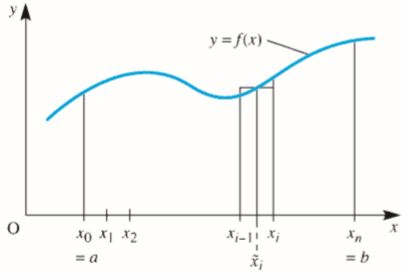
\includegraphics[scale=0.6]{Integral.JPG}
    \caption{Definite integral as an area}
\end{figure}

But that view has to be changed when \textbf{line integration} is considered since the curve $C$ is
now in a 3-D space where a scalar field $\psi(x,y,z)$ or vector field
$\textbf{\underline{F}}(x,y,z)$ has a value at \textbf{every point} within this space. 

Consider a \textbf{specific continuous curve} $C$ in 3-D space i.e. the \textbf{path of
integration} and the associated methods for summing the values of the curve within either $\psi$ or
$\textbf{\underline{F}}$. All methods rely on the fundamental definition of a curve in 3-D space: 
\begin{itemize}
    \item It always starts at a point $A$ and ends at a point $B$.
    \item On the curve, there are derived variables: arc length $\delta s$ and the chord $\delta r$
    where $O$ is the origin.
\end{itemize}

\begin{figure} [h]
\centering
\begin{subfigure}{.5\textwidth}
  \centering
  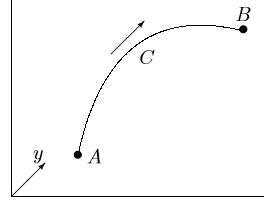
\includegraphics[width=.4\linewidth]{Line1.JPG}
  \caption{Curve in 3-D}
  \label{fig:sub1}
\end{subfigure}%
\begin{subfigure}{.5\textwidth}
  \centering
  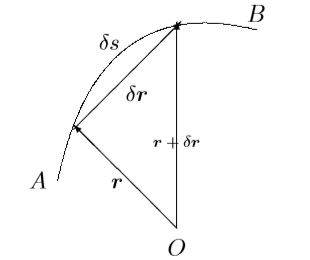
\includegraphics[width=.4\linewidth]{Line2.JPG}
  \caption{Small elements of arc length and the chord}
  \label{fig:sub2}
\end{subfigure}
\label{fig:test}
\end{figure}

The Pythagoras' Theorem in 3-D defines the the hypotenuse $\delta s$ in terms of $\delta x$, $\delta y$ and $\delta z$:
$$
    (\delta s)^2 = (\delta x)^2 + (\delta y)^2 + (\delta z)^2
$$

There are two classified types of line integral:
\begin{enumerate}
    \item Integration of a \textbf{scalar field} $\psi$ along a path $C$:
    $$
        \int_C \psi(x,y,z)\; ds
    $$

    \item Integration of a \textbf{vector field} $\textbf{\underline{F}}$ along a path $C$:
    $$
        \int_C \textbf{\underline{F}}(x,y,z)\; . \; d \textbf{r}
    $$
\end{enumerate}

\begin{tcolorbox}[breakable,colback=white]
If the curve $C$ is \textbf{closed} then the notation used is:
\begin{align*}
    \oint_C \psi(x,y,z)\; ds \\
    \oint_C \textbf{\underline{F}}(x,y,z)\; . \; d \textbf{r}
\end{align*}
where $ds = d\textbf{r} = \sqrt{dx^2+dy^2+dz^2}$ with parametrization.
\end{tcolorbox}

%%%%%%%%%%%%%%%%%%%%%%%%%%%%%%%%%%%%%%%%%%%%%%%%%%%%%%%%%%%%%%%%%%%%%%%%%%%%%%%%%%%%%%%%%%%%%%%%%%%%%%%%%%
\subsection{Integration of scalar field}

The concept is based off the arc length formula by considering:
\begin{itemize}
    \item $ds = \sqrt{dx^2+dy^2+dz^2}$ is a infinitesimal element of length.
    \item $\int_C 1\;ds$ gives the length of the curve $C$.
\end{itemize} 

\begin{tcolorbox}[breakable,colback=white]
    \begin{itemize}
        \item Recall the parametrization $x(t)$ and $y(t)$ of a curve where $a\leq t \leq b$ are the endpoints:
        $$
            \frac{ds}{dt} = \sqrt{\dot{x}^2+\dot{y}^2} \Rightarrow ds = \sqrt{\dot{x}^2+\dot{y}^2}\: dt
        $$
        \item The arc length is thus given by:
        $$
            \int_C 1 \; ds = \int_a^b \sqrt{\dot{x}^2+\dot{y}^2}\; dt
        $$
    \end{itemize}
\end{tcolorbox}

\textbf{Example 1}: Show that $\int_C x^2y \; ds = \frac{1}{3}$ where $C$ is the circular arc in the
first quadrant of the unit circle.
\begin{figure} [h]
    \centering
    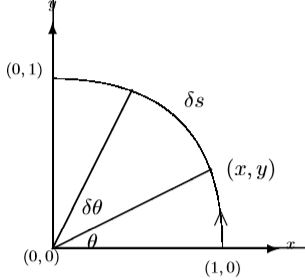
\includegraphics[scale=0.4]{Quad.JPG}
\end{figure}

\begin{enumerate}
    \item List the parameterised form:
    \begin{align*}
        x = cos(t) \Rightarrow \dot{x} = -\sin(t) \\
        y = sin(t) \Rightarrow \dot{y} = cos(t)
    \end{align*}
    \item Note the interval: 
    \begin{itemize}
        \item Question stated \textbf{first quadrant} meaning from $0$ to $\frac{\pi}{2}$.
    \end{itemize}
    \item Use previously stated arc length formula:
    \begin{align*}
        ds = \sqrt{\sin^2(t)+\cos^2(t)}\; dt = 1 \; dt 
    \end{align*}
    \item Calculate the integral:
    \begin{align*}
        \int_C x^2y \; ds &= \int_0^{\frac{\pi}{2}}\cos^2(t)\sin(t) \; dt \\
        &= \frac{1}{3}
    \end{align*}
\end{enumerate}

\textbf{Example 2}: Find $\int_C(x^2+y^2+z^2)ds$ where $C$ is the helix $r= \textbf{i} cos(t)+
\textbf{j}sin(t)+\textbf{k}t$ from $(1,0,0)$ to $(1,0,2\pi)$ and where $ds$ is an element of arc
length on $C$.
\begin{enumerate}
    \item List the parameterised form:
    \begin{align*}
        x &= cos(t) \Rightarrow \dot{x} = -\sin(t) \\
        y &= sin(t) \Rightarrow \dot{y} = cos(t) \\
        z &= t \Rightarrow \dot{z} = 1
    \end{align*}
    \item Note the interval: 
    \begin{itemize}
        \item $x$ and $y$ coordinates are not changing.
        \item $z$ coordinate is changing from $0$ to $2\pi$ which is a full revolution.
    \end{itemize}
    \item Use previously stated arc length formula:
    \begin{align*}
        \delta s = \sqrt{\sin^2(t)+\cos^2(t)} + 1 \; dt = \sqrt{2}\; dt
    \end{align*}
    \item Calculate the integral:
    \begin{align*}
        \int_C (x^2 + y^2 + z^2) \; ds &= \sqrt{2} \int_0^{2\pi} (1+t^2)\; dt \\
        &= 2\pi \sqrt{2 \left(1+\frac{4\pi^2}{3}\right)}
    \end{align*}
\end{enumerate}


\textbf{Example 3}: Show that $\int_C xy^3 \; ds = -\frac{54\sqrt{10}}{5}$ where $C$ is the line
$y=-3x$ from $x=-1 \rightarrow 1$
\begin{enumerate}
    \item List the parameterised form:
    \begin{align*}
        x &= t \Rightarrow \dot{x} = 1 \\
        y &= -3t \Rightarrow \dot{y} = -3
    \end{align*}
    \item Note the interval: 
    \begin{itemize}
        \item The question stated for the coordinate $x$ from $1$ to $-1$.
    \end{itemize}
    \item Use previously stated arc length formula:
    $$
        ds = \sqrt{\dot{x}^2 + \dot{y}^2} \; dt = \sqrt{10} \; dt
    $$
    \item Calculate the integral:
    $$
        \int_C xy^3 \; ds = \sqrt{10}\int_{-1}^1 t(-3t)^3 \; dt = -\frac{54\sqrt{10}}{5}
    $$
\end{enumerate}

%%%%%%%%%%%%%%%%%%%%%%%%%%%%%%%%%%%%%%%%%%%%%%%%%%%%%%%%%%%%%%%%%%%%%%%%%%%%%%%%%%%%%%%%%%%%%%%%%%%%%%%%%%
\subsection{Integration of vector field}

\begin{figure} [h!]
    \centering
    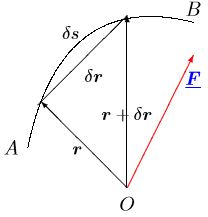
\includegraphics[scale=0.7]{Type2.JPG}
    \caption{Vector $\textbf{\underline{F}}$ and a curve $C$ with chord $\delta r$}
\end{figure}
\begin{tcolorbox}[breakable,colback=white]
    $$
    \int_C \textbf{\underline{F}}(x,y,z)\; . \; d \textbf{r}
    $$
    where $d\textbf{r} = \sqrt{dx^2+dy^2+dz^2}$
\end{tcolorbox}

\begin{itemize}
    \item \textbf{\underline{F}} is a force on a particle begin drawn through the path
    of the curve $C$.
    \item Work done $\delta W$ is the pulling of the particle along curve with arc length $\delta s$ 
    \item Chord $\delta \textbf{r}$ is $\delta W = \textbf{\underline{F}}.\delta \textbf{r}$
    $$
        W = \int_C \textbf{\underline{F}}\;.\; d \textbf{r}
    $$
\end{itemize}

Note that with the same start/end points and same integrand, the value of integral can differ with a different route.

\textbf{Example 1}: Evaluate the path of $\int_C \textbf{\underline{F}}\;.\; d \textbf{r}$ given that
$\textbf{\underline{F}}=\textbf{\underline{i}}x^2y +
\textbf{\underline{j}}(x-z)+\textbf{\underline{k}}xyz$ and two paths are
\begin{itemize}
    \item Path $C_1$ is the parabola $y=x^2$
    \item Path $C_2$ is the straight line $y=x$
\end{itemize}  
where both are in the plane where $z=2$ from $(0,0,2)$ to $(1,1,2)$

\begin{enumerate}
    \item Draw a picture of area of integration:
    \begin{figure} [h!]
        \centering
        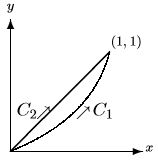
\includegraphics[scale=0.8]{Example1.JPG}
    \end{figure}
    \item Find if equations and derivatives are non-zero or not: 
    \begin{itemize}
        \item $C_1$ is along the curve in plane $z=2$:
        \begin{align*}
            dz &= 0 \\
            dy &= 2x\; dx
        \end{align*}
        \item $C_2$ is along the line $y=x$:
        \begin{align*}
            dy=dx
        \end{align*}
    \end{itemize}
    \item Find general equation $\int_{C}\textbf{\underline{F}}.d \textbf{r}$:
    \begin{align*}
        \int_{C_1}\textbf{\underline{F}}.d \textbf{r} &= \int_{C_1}(F_1\;dx + F_2\;dy + F_3\;dz)\\
        &= \int_{C_1} (x^2y \;dx + (x-z)\;dy + xyz\;dz) \\
        &= \int_{C_1} (x^2y \; dx + (x-2)\; dy)
    \end{align*}
    \item Evaluate path along $C_1$:
    Note:
    \begin{itemize}
        \item $y=x^2$, $dy=2x\;dx$ and $dz=0$
        \item Interval from $0$ to $1$
        \begin{align*}
            Path_{(C_1)} &= \int_0^1 (x^4)\;dx + (x-2)2x \; dx \\
            &= \int_0^1 (x^4 + 2x^2 - 4x)dx \\
            &= -\frac{17}{15}
        \end{align*}
    \end{itemize}

    \item Evaluate path along $C_2$:
    Note:
    \begin{itemize}
        \item Note $dy=dx$:
        \item Interval from $0$ to $1$
        \begin{align*}
            Path_{(C_2)} &= \int_0^1 (x^3\;dx + (x-2)\;dx) \\
            &= \frac{1}{4}+\frac{1}{2}-2 \\
            &= -\frac{5}{4}
        \end{align*}
    \end{itemize}
\end{enumerate}

\textbf{Example 2}: Evaluate $I=\int_C (y^2\;dx-2x^2\;dy)$ given that
$\textbf{\underline{F}}=(y^2-2x^2)$ with the path $C$ taken as $y=x^2$ in the plane $z=0$ from
$(0,0,0)$ to $(2,4,0)$.
\begin{enumerate}
    \item Draw a picture of area of integration:
    \begin{figure} [h!]
        \centering
        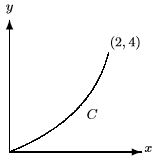
\includegraphics[scale=0.8]{Example2.JPG}
    \end{figure}
    \item Find if equations and derivatives are non-zero or not: 
    \begin{itemize}
        \item Curve $C$ defined by $y=x^2$
        \begin{align*}
            dz&=0 \\
            dy&=2x\;dx
        \end{align*}
    \end{itemize}
    \item Find general equation $\int_{C}\textbf{\underline{F}}.d \textbf{r}$:
    \begin{align*}
        \int_{C}\textbf{\underline{F}}.d \textbf{r} = \int_C (y^2\;dx-2x^2\;dy)
    \end{align*}
    \item Evaluate path along $C$
    \begin{itemize}
        \item Note $dy=2x$
        \item Interval from $0$ to $2$
        \begin{align*}
            Path_{(C)} &= \int_C (y^2\;dx-2x^2\;dy) \\
            &= \int_0^2 (x^4 - 4x^3)dx \\
            &= -\frac{48}{5}
        \end{align*}
    \end{itemize}
\end{enumerate}

\textbf{Example 3}: Find $\oint_C xy\; ds$ where $C$ is the closed path of straight lines from $(0,0)$ to
$(1,0)$ to $(0,1)$ and then back to $(0,0)$.
\begin{enumerate}
    \item Draw a picture of area of integration:
    \begin{figure} [h!]
        \centering
        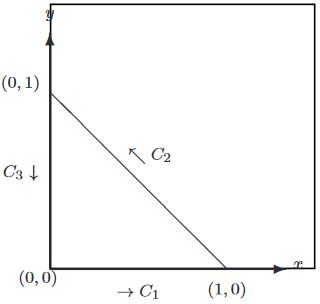
\includegraphics[scale=0.8]{Ps1.JPG}
    \end{figure}
    \item Find if equations and derivatives are non-zero or not: 
    \begin{itemize}
        \item $C_1$: $y=0$ so $ds=dx$ 
        \item $C_2$: $x=0$ so $ds=dy$ 
        \item $C_3$: $y= 1-xy$ parameterise:
        \begin{align*}
            x &= 1-t \Rightarrow \dot{x} = -1 \\
            y &= t \Rightarrow \dot{y} = 1
        \end{align*}
    \end{itemize}
    \item Find general equation $\int_{C}\textbf{\underline{F}}.d \textbf{r}$:
    \begin{align*}
        \int_{C}\textbf{\underline{F}}.d \textbf{r} = \int_C xy \; d\textbf{r}
    \end{align*}
    where $d\textbf{r} = \sqrt{\dot{x}^2 + \dot{y}^2 + \dot{z}^2 \; dt}$
    \item Evaluate path along $C$
    \begin{itemize}
        \item $C_1$
        $$
        \int_{C_1}xy \; ds= 0.
        $$
        \item $C_2$
        Note:
        \begin{itemize}
            \item Interval of $y$ from $0$ to $1$.
            \item $d\textbf{r} = \sqrt{\dot{x}^2 + \dot{y}^2 + \dot{z}^2\; dt} = \sqrt{2}\; dt$
        \end{itemize}
        \begin{align*}
            \int_{C_2}xy \; ds= \sqrt{2}\int_0^1 (1-t)t\; dt = \frac{\sqrt{2}}{6}
        \end{align*}
        \item $C_3$
        $$
        \int_{C_3}xy \; ds= 0.
        $$
    \end{itemize}
    \item Sum $C_1$, $C_2$ and $C_3$:
    \begin{align*}
        \oint xy \; ds = \frac{\sqrt{2}}{6}
    \end{align*}
\end{enumerate}

%%%%%%%%%%%%%%%%%%%%%%%%%%%%%%%%%%%%%%%%%%%%%%%%%%%%%%%%%%%%%%%%%%%%%%%%%%%%%%%%%%%%%%%%%%%%%%%%%%%%%%%%%%
\subsubsection{Path independence and Fundamental theorem of line integrals}

There are circumstances where a line integral $\int_C \textbf{\underline{F}}.d \textbf{r}$ takes
values which are \textbf{independent of the path $C$}.

\begin{tcolorbox}[breakable,colback=white]
\textbf{Theorem}: Assuming that $C$ is a smooth curve given by $$r(t) - a\leq t \leq b$$

$f$ is a function whose gradient vector $\nabla\;f$ is continuous on $C$:
$$
    \int_C \nabla f\;.\;dr = f[r(b)]-f[r(a)]
$$
\end{tcolorbox}

\textbf{Proof}:
\begin{enumerate}
    \item Compute the line integral:
    \begin{align*}
        \int_C \nabla f\;.\;d \textbf{r} &= \int_a^b \nabla f[r(t)].r(t)\; dt \\
        &= \int_a^b \left(\frac{\partial f}{\partial x}\frac{dx}{dt}+\frac{\partial f}{\partial y}\frac{dy}{dt}+\frac{\partial f}{\partial z}\frac{dz}{dt}\right) dt
    \end{align*}
    \item Use Chain Rule to simplify the integrand:
    \begin{align*}
        \int_C \nabla f\;.\;d \textbf{r} &= \int_a^b \left(\frac{\partial f}{\partial x}\frac{dx}{dt}+\frac{\partial f}{\partial y}\frac{dy}{dt}+\frac{\partial f}{\partial z}\frac{dz}{dt}\right) dt \\ 
        &= \int_a^b \frac{d}{dt}[f[r(t)]] dt 
    \end{align*}
    \item Fundamental Theorem of Calculus for single integrals:
    \begin{align*}
        \int_C \nabla f\;.\;dr = f[r(b)]-f[r(a)]
    \end{align*}
\end{enumerate}

A \textbf{conservative vector field} (path-independent vector field) is a function such that $F = \nabla f$
where $f$ is the \textbf{potential function} for the vector field i.e. a curl-free vector field
$\textbf{\underline{F}}$. 

\begin{tcolorbox}[breakable,colback=white]
    \textbf{Independence of path}: If $\int_{(C_1)}F\;.\;dr = \int_{(C_2)}F\;.\;dr $ for any
    two paths $C_1$ and $C_2$ in $D$ with the same initial and final points.
    \\
    \\
    If integral $\int_C \textbf{\underline{F}}\;.\;d \textbf{r}$ is independent of path then its
    path is curl free since $C$ is closed i.e. start point and end point are the same:
    $$
        \text{curl }\textbf{\underline{F}} = 0
    $$
\end{tcolorbox}

\textbf{Example 1}: Evaluate if line integral $\int_C (2xy^2\; dx + 2x^2y\; dy)$ is independent of
path.

\begin{enumerate}
    \item Express line integral as:
    $$\textbf{\underline{F}}=2xy^2\textbf{\underline{i}}+2x^2y\textbf{\underline{j}}+0\textbf{\underline{k}}$$
    \item Find the curl $\textbf{\underline{F}}$: 
    \begin{align*}
        \text{curl }\textbf{\underline{F}} &= 
        \begin{bmatrix}
            \textbf{\underline{i}} & \textbf{\underline{j}} & \textbf{\underline{k}} \\
            \partial_x & \partial_y & \partial_z \\
            2xy^2 & 2x^2y & 0
        \end{bmatrix}\\ &= (4xy - 4xy)\textbf{\underline{k}} \\ &= 0
    \end{align*}
\end{enumerate}

\textbf{Example 2}: Find work done $\int_C \textbf{\underline{F}}\;.\; d \textbf{r}$ by the force
$\textbf{\underline{F}}=(yz,xz,xy)$ moving from $(1,1,1) \rightarrow (3,3,2)$.
\begin{enumerate}
    \item Check if line integral is independent of path i.e. if curl $\textbf{\underline{F}}=0$:
    \begin{align*}
        \text{curl}\;\textbf{\underline{F}} = \begin{bmatrix}
            \textbf{\underline{i}} & \textbf{\underline{j}} & \textbf{\underline{k}} \\
            \partial_x & \partial_y & \partial_z \\
            yz & xz & xy
        \end{bmatrix} = 0
    \end{align*}

    \item Calculate $\phi$ from $\textbf{\underline{F}}=-\nabla\phi$:
    \begin{align*}
        -\frac{\partial \phi}{\partial x} = yz \;&\Rightarrow \;\phi = -xyz + A(y,z)\\
        -\frac{\partial \phi}{\partial y} = xz \;&\Rightarrow \;\phi = -xyz + B(x,z)\\
        -\frac{\partial \phi}{\partial z} = xy \;&\Rightarrow \;\phi = -xyz + C(x,y)
    \end{align*}
    Since $A(y,z) = B(x,z) = C(x,y) = \text{const}$
    \begin{align*}
        \phi = -xyz + C
    \end{align*}

    \item Calculate the work:
    \begin{align*}
        W &= - \int_{(1,1,1)}^{(3,3,2)} 1 \; d\phi \\
        &= [xyz]_{(1,1,1)}^{(3,3,2)} \\
        &= 18 -1 \\
        &= 17
    \end{align*}
\end{enumerate}

\textbf{Example 3}: Evaluate the line integrals for the following:
\begin{align*}
    I_1 &= \int_C \left[y^2 \cos(x)dx + 2y\sin(x)dy\right] \\
    I_2 &= \int_C \left[2y^2 dx - x dy\right]
\end{align*}
\begin{itemize}
    \item $C$ is the straight line between $(0,0)$ and $(\frac{\pi}{2},1)$
    \item $C$ is the straight line from $(0,0)$ to $(\frac{\pi}{2},0)$ and a line from
    $(\frac{\pi}{2},0)$ to $(\frac{\pi}{2},1)$
\end{itemize}

Why is $I_1$ equal for both $C$ but not $I_2$?

\begin{enumerate}
    \item Draw a picture of area of integration:
    \begin{figure} [h!]
        \centering
        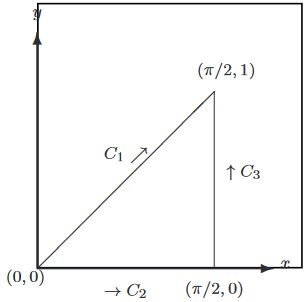
\includegraphics[scale=0.6]{Inde_ex.JPG}
    \end{figure}
    \item Evaluate $I_1$:
    \begin{enumerate}
        \item Test if independent or not:
        \begin{gather*}
            F_1 = y^2\cos(x) \; \text{ and }\; F_2 = 2y\sin(x) \\
            F_{1,y} = F_{2,x} = 2y\cos(x) \\
            \Rightarrow I_1 \text{ is independent}
        \end{gather*}
        \item If $I_1$ is independent, $I_1$ over $C_1$ is equal to $I_1$ over $C_2 + C_3$:
        \begin{align*}
            I_1 &= \int_{C_1}\left[y^2\cos(x)\; dx + 2y\sin(x)\; dy\right] \\
            &= \int_{C_1} d(y^2\sin(x)) \\
            &= [y^2\sin(x)]_{(0,0)}^{(\frac{\pi}{2},1)} \\
            &= 1
        \end{align*}
    \end{enumerate}
    \item Evaluate $I_2$:
    \begin{enumerate}
        \item Test if independent or not:
        \begin{gather*}
            F_1 = 2y^2 \; \text{ and }\; F_2 = -x \\
            F_{1,y} \neq F_{2,x} \\
            \Rightarrow I_1 \text{ is not independent}
        \end{gather*}
        \item Evaluate over $C_1$ i.e. along the line $y=\frac{2}{\pi}x$:
        \begin{align*}
            \int_{C_1} (2y^2\; dx - x\; dy) &= \int_0^{\frac{\pi}{2}}\left[2\left(\frac{2}{\pi}\right)^2 x^2 - \frac{2}{\pi}x\right]dx \\ 
            &= \frac{\pi}{3} - \frac{\pi}{4} \\
            &= \frac{\pi}{12}
        \end{align*} 
        \item Evaluate over $C_2$ (line $y=0 \Rightarrow dy = 0$) then over $C_3$ (line
        $x=\frac{\pi}{2} \Rightarrow dx = 0$):
        \begin{align*}
            \int_{{C_2}+{C_3}} &= int_{C_2} + \int_{C_3} \\
            &= \int_{C_2}(2y^2\:dx - x\: dy) + \int_{C_3}(2y^2\:dx - x\: dy) \\
            &= 0 - \frac{\pi}{2}\int_0^1 \\
            &= -\frac{\pi}{2}
        \end{align*}
        \item $\int_{C_1}\neq \int_{{C_2}+{C_3}}$ since $I_2$ is not independent.
    \end{enumerate}
\end{enumerate}

\pagebreak
%%%%%%%%%%%%%%%%%%%%%%%%%%%%%%%%%%%%%%%%%%%%%%%%%%%%%%%%%%%%%%%%%%%%%%%%%%%%%%%%%%%%%%%%%%%%%%%%%%%%%%%%%%
\section{Double and Multiple Integration}

In the previous sections, the \textbf{definite integral of a function $f(x)$} of one variable by the limit
defined:
$$
    \int_b^a f(x)\; dx = \lim_{\substack{n\rightarrow\infty \\ \text{all }\Delta x_i \rightarrow 0}} \sum_{i=1}^n f(x_i)\Delta x_i
$$
where \begin{itemize}
    \item $a=x_0<x_1<x_2<\dots<x_n = b$
    \item $\Delta x_i = x_i - x_{i-1}$
\end{itemize}

\begin{figure} [h!]
    \centering
    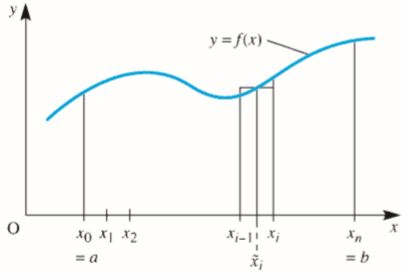
\includegraphics[scale=0.6]{Integral.JPG}
    \caption{Graphical definition of definite integral}
\end{figure}

Considering the region $R$ in the $x-y$ plane with boundary curve $C$, the integral of $f(x,y)$ is
defined as \textbf{"the double integral of $\psi$ over the region $R$"}:

\begin{figure} [h!]
    \centering
    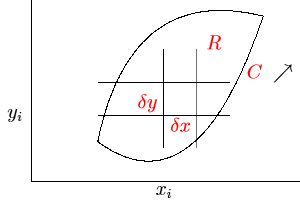
\includegraphics[scale=0.65]{Doubleint.JPG}
\end{figure}
\begin{align*}
    \sum_{i=1}^N \sum_{j=1}^M \psi(x_i,y_i) \delta A_i \rightarrow \int \int_R \psi(x,y) \: dxdy \; \text{as } \delta x \rightarrow 0 \text{ and } \delta y \rightarrow 0
\end{align*}
where:
\begin{itemize}
    \item $\psi(x_i,y_i)$ is the value of a scalar function at the point $(x_i,y_i)$
    \item The area denoted as $\delta A_i = \delta x_i \delta y_i$
\end{itemize}

\pagebreak
\textbf{Note}: There is a fundamental difference between "Double integral of $\psi$ over the region
$R$" and "Area of $R$" which is defined as $\text{Area of R} = \int \int_R dxdy$

\begin{figure}[h]
\centering
\begin{subfigure}{.5\textwidth}
  \centering
  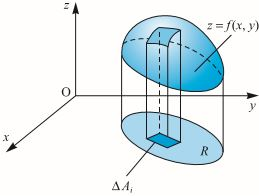
\includegraphics[width=.6\linewidth]{Diff.JPG}
  \caption{Double integral of $\psi$ over the region $R$}
  \label{fig:sub1}
\end{subfigure}%
\begin{subfigure}{.5\textwidth}
  \centering
  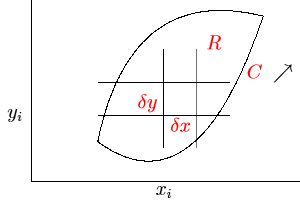
\includegraphics[width=.6\linewidth]{Doubleint.JPG}
  \caption{Area of $R$}
  \label{fig:sub2}
\end{subfigure}
\caption{Difference between the two statements as aforementioned}
\label{fig:test}
\end{figure}

\textbf{Working example}:

\begin{figure} [h!]
    \centering
    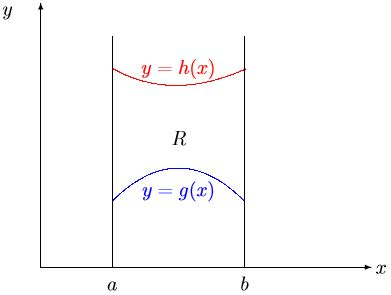
\includegraphics[scale=0.6]{How.JPG}
\end{figure}

Region $R$ is bounded between the upper curve ($y=h(x)$), lower curve ($y=g(x)$), line $x=a$ and
line $x=b$.
$$
    \int \int_R \psi(x,y)\; dxdy = \int_a^b \left\{\int_{y=g(x)}^{y=h(x)}\psi(x,y)\;dy\right\} dx
$$

Given that the inner integral is a partial integral over $y$ holding $x$ constant - the inner
integral is a function of $x$:
$$
    \int_{y=g(x)}^{y=h(x)} \psi(x,y)dy = P(x)
$$
Thus can be simplified into:
$$
    \int \int_R \psi(x,y)\; dxdy = \int_a^b P(x)\; dx
$$

\begin{tcolorbox}[breakable,colback=white]
Area of $R$:
$$
    \text{Area of R} = \int_a^b\left\{\int_{y=g(x)}^{y=h(x)} dy\right\} dx = \int_a^b \{h(x)-g(x)\}\; dx
$$
\end{tcolorbox}

%%%%%%%%%%%%%%%%%%%%%%%%%%%%%%%%%%%%%%%%%%%%%%%%%%%%%%%%%%%%%%%%%%%%%%%%%%%%%%%%%%%%%%%%%%%%%%%%%%%%%%%%%%
\subsection{Applications of double integration}

\begin{enumerate}
    \item Area under a curve
    For a function of a single variable $y=f(x)$ between $x=a$ and $x=b$:
    $$
        \text{Area} = \int_a^b \left\{\int_0^{f(x)}dy\right\}dx = \int_a^b f(x) \; dx
    $$
    \item Volume under a surface
    A surface is 3-D space may be expressed as $z=f(x,y)$:
    \begin{align*}
        \text{Volume}&=\int \int \int_V dx\;dy\;dz\\
        &= \int_R \left\{\int_0^{f(x,y)}dz\right\}dxdy \\
        &= \int \int_R f(x,y)dx\;dy
    \end{align*}
    This process reduces a 3-integral into a double integral
    \item Mass of a solid body
    Let $p(x,y,z)$ be the variable density of the material in a solid body. Mass $\delta M$ of
    a small volume $\delta V = \delta x \delta y \delta z$ is $\delta M = \rho \delta V$:
    $$
        \text{Mass of body} = \int \int \int_V p(x,y,z) dV
    $$
\end{enumerate}

\textbf{Example 1}: Consider the first quadrant circle of radius $a$:
\begin{figure*} [h!]
    \centering
    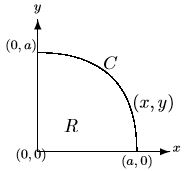
\includegraphics[scale=0.7]{Ex3.JPG}
\end{figure*}

Show that:
\begin{enumerate}
    \item Area of $R = \frac{\pi a^2}{4}$
    
    The area of $R$ is given by:
    \begin{align*}
        A &= \int_0^a \left\{\int_0^{\sqrt{a^2-x^2}}dy\right\}dx \\
        &= \int_0^a \sqrt{a^2-x^2}dx
    \end{align*}

    Let $x=a\cos(\theta)$ and $dx=-a\sin(\theta) d\theta$:
    \begin{align*}
        A &= \frac{1}{2}a^2 \int_0^{\frac{\pi}{2}}(1-\cos(2\theta))d\theta \\
        &= \frac{\pi a^2}{4}
    \end{align*}

    \item $\int \int_R xy \; dxdy = \frac{a^4}{8}$
    
    \begin{align*}
        \int \int_R xy \; dxdy &= \int_0^a x \left(\int_0^{\sqrt{a^2-x^2}}y \; dy\right)dx \\
        &= \frac{1}{2}\int_0^a x(a^2 - x^2) dx \\
        &= \frac{1}{2}[\frac{1}{2}x^2a^2 - \frac{1}{4}x^4]_0^a \\
        &= \frac{a^4}{8} 
    \end{align*}

    \item $\int \int_R x^2y^2 \; dxdy = \frac{\pi a^6}{96}$
    
    \begin{align*}
        \int \int_R x^2y^2 \; dxdy &= \int_0^a x^2 \left(\int_0^{\sqrt{a^2-x^2}}y^2 \; dy\right) dx \\
        &= \frac{1}{3} \int_0^a x^2(a^2-x^2)^{\frac{3}{2}} dx \\
        &= \frac{1}{3} a^6 \int_0^{\frac{\pi}{2}} \cos^2(\theta)\sin^4(\theta) d\theta \\
        &= \frac{1}{3}a^6(I_4 - I_6)
    \end{align*}
    where $I_n = \int_0^{\frac{\pi}{2}}\sin^n(\theta)d\theta$ which is an integral recurrence
    relation:
    $$
        I_n=\left(\frac{n-1}{n}\right)I_{n-2} \dots I_2 = \frac{\pi}{4} \dots I_4 = \frac{3\pi}{16} \dots I_6 = \frac{5\pi}{32}
    $$
    Thus substituting in the values of $I_n$:
    $$
        \frac{1}{3}a^6(I_4 - I_6) = \frac{\pi a^6}{96}
    $$
\end{enumerate}

%%%%%%%%%%%%%%%%%%%%%%%%%%%%%%%%%%%%%%%%%%%%%%%%%%%%%%%%%%%%%%%%%%%%%%%%%%%%%%%%%%%%%%%%%%%%%%%%%%%%%%%%%%
\subsection{Changing order of double integration}

Sometimes changing the order of integration makes evaluations much easier. For example: $I=\int_0^a
\left(\int_y^a \frac{x^2\; dx}{x^2+y^2}\right)dy$. 

Process of changing order of double integration:
\begin{enumerate}
    \item Deduce the area of integration from the internal limits:
    
    The internal integral (from the above example):
    $$
        \int_{x=y}^{x=a}f(x,y)\; dx
    $$

    The \textbf{left limit} is $x=y$ and the \textbf{right limit} is $x=a$.

    \item Draw the graph showing the \textbf{region of integration} $R$:
    \begin{figure} [h!]
        \centering
        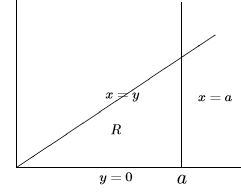
\includegraphics[scale=0.75]{R.JPG}
        \caption{Region of Integration labelled $R$}
    \end{figure}

    \item Perform integration over $R$ but in reverse order: Integrate \textbf{vertically} then \textbf{horizontally}
    \begin{itemize}
        \item Lower vertical limit: $y=0$
        \item Upper vertical limit: $y=x$
        \item Lower horizontal limit: $x=0$
        \item Upper horizontal limit: $x=a$
    \end{itemize}
    $$
        I = \int_{x=0}^{x=a} \left(\int_{y=0}^{y=x}\frac{x^2 \; dy}{x^2+y^2}\right) dx
    $$

    \item Inner integrate before using the result to outer integrate:
    \begin{align*}
        &\text{Inner integration: } \int_0^x \frac{x^2\; dy}{x^2+y^2} = x\int_0^1 \frac{d\theta}{1+\theta^2} = \frac{\pi x}{4} \\
        &\text{Outer integration: } I = \frac{\pi}{4}\int_0^a x\; dx = \frac{\pi a^2}{8}
    \end{align*} 
\end{enumerate}

%%%%%%%%%%%%%%%%%%%%%%%%%%%%%%%%%%%%%%%%%%%%%%%%%%%%%%%%%%%%%%%%%%%%%%%%%%%%%%%%%%%%%%%%%%%%%%%%%%%%%%%%%%
\subsection{Change of variable and Jacobian}

Sometimes it is easier to deal with the natural circular symmetry in the problem by changing the
order of the variables. This requires expressions in polar co-ordinates. 

\begin{figure*}
\centering
\begin{subfigure}{.5\textwidth}
  \centering
  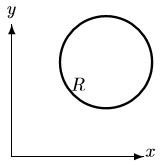
\includegraphics[width=.4\linewidth]{Jacob1.JPG}
  \caption{Region $R$ in $x-y$ plane}
  \label{fig:sub1}
\end{subfigure}%
\begin{subfigure}{.5\textwidth}
  \centering
  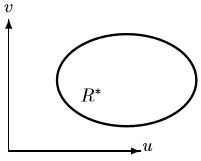
\includegraphics[width=.4\linewidth]{Jacob2.JPG}
  \caption{Distorted region $R*$ in plane of new coordinates $u=u(x,y)$ and $v=v(x,y)$}
  \label{fig:sub2}
\end{subfigure}
\label{fig:test}
\end{figure*}

\begin{tcolorbox}[breakable,colback=white]
    \textbf{Theorem 1}:

    The transformation relates the two small areas $\delta x \delta y$ and $\delta u \delta v$:
    $$
        dxdy = |J_{u,v}(x,y)| dudv
    $$
    where the Jacobian $J_{u,v}(x,y)$ is defined:
    $$
        J_{u,v}(x,y) = 
        \begin{bmatrix}
            \frac{\partial x}{\partial u} & \frac{\partial x}{\partial v} \\
            \frac{\partial y}{\partial u} & \frac{\partial y}{\partial v}
        \end{bmatrix}
    $$

    Note: 
    \begin{itemize}
        \item $\frac{\partial x}{\partial u} \neq \left(\frac{\partial u}{\partial x}\right)^{-1}$
        \item $J_{x,y}(u,v) = \left[J_{u,v}(x,y)\right]^{-1}$
        \item $dudv = |J_{x,y}(u,v)|dxdy$
    \end{itemize}
\end{tcolorbox}

\begin{tcolorbox}[breakable,colback=white]
\textbf{Theorem 2}: 

Inverse relationship can be proved in a similar manner:
$$
    \int \int_R f(x,y)\; dxdy = \int \int_{R*} f[x(u,v),y(u,v)]|J_{u,v}(x,y)|\; dudv
$$
\end{tcolorbox}

\textbf{Example 1}: For polar coordinates $x=r\cos(\theta)$ and $y=r\sin(\theta)$, take $u=r$ and
$v=\theta$:
$$
    J_{r,\theta}(x,y) = 
    \begin{bmatrix}
        \frac{\partial x}{\partial r} & \frac{\partial x}{\partial \theta} \\
        \frac{\partial y}{\partial r} & \frac{\partial y}{\partial \theta} 
    \end{bmatrix} = 
    \begin{bmatrix}
        \cos(\theta) & -r\sin(\theta) \\
        \sin(\theta) & r\cos(\theta)
    \end{bmatrix} = r
$$
Thus:
$$
    dxdy = r\; drd\theta
$$

\textbf{Example 2}: Calculate the volume of a sphere of radius $a$, note that $z=\pm \sqrt{a^2 - x^2
- y^2}$.
\begin{enumerate}
    \item Double up the two hemisphere:
    $$
        \text{Volume} = 2\int\int_R \sqrt{a^2 - x^2 - y^2} dxdy 
    $$
    where $R$ is the disc $x^2+y^2 \leq a^2$ in the $z=0$ plane

    \item Use a change of variable:
    \begin{align*}
        \text{Volume} &= 2\int \int_R \sqrt{a^2 - x^2 - y^2} dxdy \\
        &= 2 \int \int_R \sqrt{a^2 - r^2}r \; drd\theta \\
        &= 2 \int_0^a \sqrt{a^2 - r^2}r \; dr \int_0^{2\pi}d\theta \\
        &= \frac{4\pi a^3}{3}
    \end{align*}
\end{enumerate}

\textbf{Example 3}: Show that $\int \int_R (x^2 + y^2) dxdy = \frac{8}{3}$ using $u=x+y$ and
$v=x-y$:
\begin{itemize}
    \item Where $R$ has corners at $(0,0)$, $(1,1)$, $(2,0)$ and $(1,-1)$.
    \item Rotates to a square with corners at $(0,0)$, $(2,0)$, $(2,2)$ and $(0,2)$.
\end{itemize}

Process:
\begin{enumerate}
    \item From $x=\frac{1}{2}(u+v)$ and $y=\frac{1}{2}(u-v)$:
    $$
        J_{u,v}(x,y) = -\frac{1}{2}
    $$
    \item Solve:
    \begin{align*}
        I &= \frac{1}{4} \int \int_{R*} 2(u^2+v^2)|-\frac{1}{2}|\; dudv \\
        &= \frac{1}{4} \left\{[\frac{1}{3}u^3]_0^2 [v]_0^2 + [\frac{1}{3}v^3]_0^2[u]_0^2\right\} \\
        &= \frac{8}{3}
    \end{align*}
\end{enumerate}

%%%%%%%%%%%%%%%%%%%%%%%%%%%%%%%%%%%%%%%%%%%%%%%%%%%%%%%%%%%%%%%%%%%%%%%%%%%%%%%%%%%%%%%%%%%%%%%%%%%%%%%%%%
\section{Green's Theorem (in a plane)}

The relationship between certain kinds of line integrals on closed paths and double integrals is
investigated. This relationship is illustrated with a simple closed curve $C$ i.e. does not cross
itself and let $D$ be the region enclosed by the curve:
\begin{figure} [h!]
    \centering
    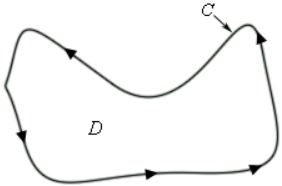
\includegraphics[scale=0.6]{Intro green.JPG}
\end{figure}

Note that a direction has been put on the curve - the convention used is that the curve $C$ has a
\textbf{positive orientation} that is traced out in a \textbf{counter-clockwise direction}. 

%%%%%%%%%%%%%%%%%%%%%%%%%%%%%%%%%%%%%%%%%%%%%%%%%%%%%%%%%%%%%%%%%%%%%%%%%%%%%%%%%%%%%%%%%%%%%%%%%%%%%%%%%%
\subsection{Intuition behind Green's theorem}

When $C$ is an oriented simple closed curve, the integral $\int_C \textbf{F}\;.\;ds$ represents the
circulation of $\textbf{F}$ around $C$ e.g. if $\textbf{F}$ were the velocity field of water flow,
the integral would indicate how much the water tends to circulate around the path in the direction
of its orientation. \par

One way to compute this circulation is to compute the line integral directly. But, if the line
integral is two dimensional i.e. $\textbf{F}$ is a two-dimensional vector field and $C$ is a closed path that
lives in the plane, then Green's theorem can be used as an alternative way to calculate the line integral.

Think of the integral $\int_C \textbf{F}\;.\;ds$  as the \textbf{macroscopic circulation} of the
vector field $\textbf{F}$ around the path $C$. \par
\begin{figure} [h!]
    \centering
    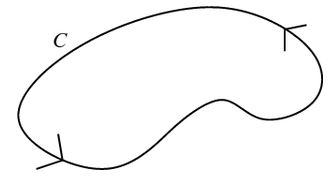
\includegraphics[scale=0.6]{flow.JPG}
\end{figure}
There is a \textbf{microscopic version of circulation} around a curve at a point $(x,y)$ that shows
how much $\textbf{F}$ would circulate around a tiny closed curve centered around $(x,y)$. \par
\begin{figure} [h!]
    \centering
    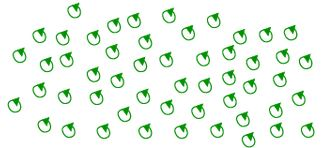
\includegraphics[scale=0.6]{micro.JPG}
\end{figure}
Green's theorem is a relationship between the macroscopic circulation around the curve $C$ and the
sum of all the microscopic circulation that is inside $C$. The \textbf{sum of the microscopic circulation} inside
$C$ i.e. the microscopic circulation in $D$ is exactly the same as the \textbf{macroscopic
circulation} around $C$. \par
\begin{figure} [h!]
    \centering
    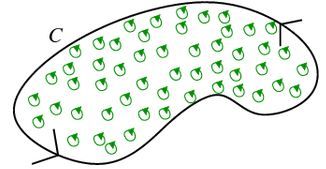
\includegraphics[scale=0.6]{combined.JPG}
\end{figure}
The microscopic circulation of Green's theorem is the same as the curl of a three-dimensional vector
field in the $z$-direction (Refer to right hand rule in curl). Thus be careful on the orientation of
the curve $C$. The right hand rule says that the orientation corresponds to the \textbf{counterclockwise direction}.

%%%%%%%%%%%%%%%%%%%%%%%%%%%%%%%%%%%%%%%%%%%%%%%%%%%%%%%%%%%%%%%%%%%%%%%%%%%%%%%%%%%%%%%%%%%%%%%%%%%%%%%%%%
\subsection{Formal statement of Green's theorem}

Let $R$ be a closed region that is bounded in the $x-y$ plane with piecewise
smooth boundary $C$. $P(x,y)$ and $Q(x,y)$ are continuous functions \textbf{within} $R$ that has continuous
partial derivatives $Q_x$ and $P_y$ respectively.

\begin{figure*}[h]
    \centering
    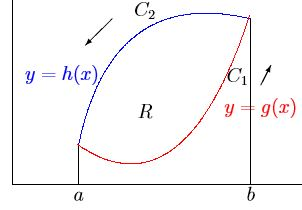
\includegraphics[]{Greens.JPG}
\end{figure*}

\begin{tcolorbox}[breakable,colback=white]
\textbf{Green's Theorem}
$$
    \oint_C (P\;dx + Q \; dy) = \int \int_R (Q_x - P_y)\;dxdy = \int\int_A \left(\frac{\partial Q}{\partial x}-\frac{\partial P}{\partial y}\right)\; dxdy 
$$
\end{tcolorbox}

\textbf{Proof}: With reference to the diagram, $R$ is bounded by upper and lower boundaries:
$g(x)\leq y \leq h(x)$:
\begin{enumerate}
    \item Perform double integration for $P$:
    \begin{align*}
        -\int \int_R \frac{\partial P}{\partial y}\; dxdy &= -\int_a^b \left\{\int_{y=g(x)}^{y=h(x)}\frac{\partial P}{\partial y}\; dy\right\}\; dx \\
        &= -\int_a^b \{P(x,\; h(x)) - P(x,\; g(x))\}\; dx \\ 
        \text{(Switch limits and signs)} &= \int_a^b P(x,\; g(x))\; dx + \int_b^a P(x,\; h(x))\;dx \\
        &= \int_{C1}P(x,\; y)\; dx + \int_{C2}P(x,\; y)\; dx \\
        &= \oint_C P(x,\; y) \; dx 
    \end{align*}

    \item Perform the same double integration for $Q$
    \item Combine both results:
    \begin{align*}
        \int \int_C \left(\frac{\partial Q}{\partial x} - \frac{\partial P}{\partial y}\right)\; dxdy = \oint_C [P(x,\;y)\; dx + Q(x,\; y)\; dy]
    \end{align*}
\end{enumerate}

\textbf{Example 1}: Use Green's Theorem to evaluate the line integral: 
$$\oint_C \{(x-y)dx - x^2dy\}$$
where $R$ and $C$ are given by:
\begin{figure} [h!]
    \centering
    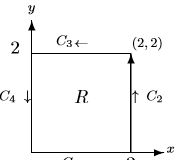
\includegraphics[]{Gex1.JPG}
\end{figure}

\begin{enumerate}
    \item Note the provided diagram and the orientation.
    \item Establish $P$ and $Q$ 
    \begin{align*}
        P = x - y \; \text{ and } \; Q = -x^2
    \end{align*}
    \item Find $\frac{\partial P}{\partial y}$ and $\frac{\partial Q}{\partial x}$:
    \begin{align*}
        \frac{\partial P}{\partial y} = -1 \; \text{ and } \; \frac{\partial Q}{\partial x} = -2x
    \end{align*}
    \item Use Green's theorem and split $x$ and $y$ respectively:
    \begin{align*}
        \oint_C \{(x-y)dx - x^2dy\} &= \int\int_A \left(\frac{\partial Q}{\partial x}-\frac{\partial P}{\partial y}\right)\; dxdy \\
        &= \int \int_R (1-2x)\; dxdy \\
        &= \int_0^2 dy \int_0^2 (1-2x) \; dx \\
        &= -4
    \end{align*}
    \item Direct valuations results in:
    $$
        \oint_C = \int_{C_1} + \int_{C_2} + \int_{C_3} + \int_{C_4}
    $$
    where:
    \begin{align*}
        C_1&: y = 0 \\
        C_2&: x = 2 \\
        C_3&: y = 2 \\
        C_4&: x = 0
    \end{align*}
    \item Combine:
    \begin{align*}
        \oint_C &= \int_0^2 x\; dx -4\int_0^2 dy + \int_2^0(x-2)\; dx + 0 \\
        &= 2 - 8 + 2 \\
        &= -4
    \end{align*}
\end{enumerate}

\textbf{Example 2}: Use Green’s Theorem to convert the line integral $\oint_C
[6xy\:dx+(2x^3y+3x^2)dy]$ where $C$ is the triangle with vertices $(0, 0)$, $(1, 1)$ and $(0, 1)$ into double integrals and hence evaluate it:

Process:
\begin{enumerate}
    \item Draw the diagram and label orientation:
    \begin{figure} [h!]
        \centering
        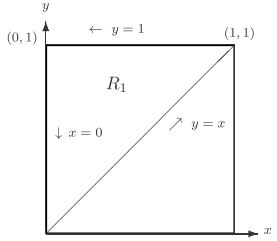
\includegraphics[scale=0.7]{Ex2.2.JPG}
    \end{figure}
    \item Establish $P$ and $Q$ 
    \begin{align*}
        P = 6xy \; \text{ and } \; Q = 2x^3y+3x^2
    \end{align*}
    \item Find $\frac{\partial P}{\partial y}$ and $\frac{\partial Q}{\partial x}$:
    \begin{align*}
        \frac{\partial P}{\partial y} = 6x \; \text{ and } \; \frac{\partial Q}{\partial x} = 6x^2y+6x
    \end{align*}
    \item Use Green's theorem and split $x$ and $y$ respectively:
    \begin{align*}
        \oint_C \{(x-y)dx - x^2dy\} &= \int\int_A \left(\frac{\partial Q}{\partial x}-\frac{\partial P}{\partial y}\right)\; dxdy \\
        &= 6\int \int_{R_1} x^2y \: dxdy \\
        &= 6\int_0^1 x^2 \left(\int_{y=x}^{y=1}y\: dy\right) \: dx \\
        &= 3\int_0^1 x^2(1-x^2)\:dx \\
        &= \frac{2}{5}
    \end{align*}
\end{enumerate}

%%%%%%%%%%%%%%%%%%%%%%%%%%%%%%%%%%%%%%%%%%%%%%%%%%%%%%%%%%%%%%%%%%%%%%%%%%%%%%%%%%%%%%%%%%%%%%%%%%%%%%%%%%
\section{Surface Integrals}

The extension of the idea of computing the integral of a vector field on a surface.

\begin{tcolorbox}[breakable,colback=white]
    $$
        \int \int_S \textbf{F(r)}\;.\;d\textbf{S} = \int \int_S \textbf{F(r)}\;.\;\hat{\textbf{n}}\; dS  
    $$
\end{tcolorbox}

\begin{tcolorbox}[breakable,colback=white]
\textbf{Note}:
\begin{itemize}
    \item $d \textbf{S}=\hat{\textbf{n}}dS$ - The vector element of area
    \item $\hat{\textbf{n}}$ - Unit outward-drawn normal vector to the element $dS$
    \item $dS$ - Infinitesimal area patch on the surface
\end{itemize}
\end{tcolorbox}

Such integrals are called \textbf{flux integrals} and gives the flux of the vector field through the
surface $S$ e.g. if the vector field is the flow of water then the flux is the \textbf{volume} of
water flowing through $S$ per unit time.

%%%%%%%%%%%%%%%%%%%%%%%%%%%%%%%%%%%%%%%%%%%%%%%%%%%%%%%%%%%%%%%%%%%%%%%%%%%%%%%%%%%%%%%%%%%%%%%%%%%%%%%%%%
\subsection{Guass' (Divergence) Theorem}

In the same way the Green's Theorem relates surface and line integrals, Gauss's theorem relates
surface and volume integral. It allows the conversion of \textbf{surface integrals} into
\textbf{volume integrals} thus simplifying the evaluation. Green's Theorem is a 2-D version of Gauss's Theorem:
\begin{align*}
    \int \int_R \text{div }\textbf{u}\; dxdy = \oint_C \textbf{u}\; . \; \hat{\textbf{n}}\; ds
\end{align*}
The line integral expresses the sum of the normal component of $\textbf{u}$ around the boundary. If
$\textbf{u}$ is a solenoid vector (an incompressible vector field i.e. a divergence-free vector field) $(\text{div }\textbf{u}=0)$ then $\oint_C \textbf{u}\; . \;
\hat{\textbf{n}}\; ds = 0$.

\begin{tcolorbox}[breakable,colback=white]
\textbf{Gauss's Theorem (3-D)}: 
\begin{align*}
    \int \int \int_V \text{div }\textbf{u}\;dV = \int\int_S \textbf{u}\;.\;\hat{\textbf{n}}\; dS
\end{align*}
or
\begin{align*}
    \int \int \int_V \nabla \; .\;\textbf{u}\; dV = \int \int_S \textbf{u}\; .\; d\overrightarrow{S}
\end{align*}
\end{tcolorbox}

The theorem uses a 3-D vector field $\textbf{u}(x,y,z)$ that exists in some finite volume $V$ whose
surface is $S$ - $dS$ is some small element of are on the curved, closed surface $S$.
\begin{figure} [h!]
    \centering
    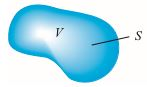
\includegraphics[]{Gauss.JPG}
    \caption{Closed volume $V$ with surface $S$}
\end{figure}

%%%%%%%%%%%%%%%%%%%%%%%%%%%%%%%%%%%%%%%%%%%%%%%%%%%%%%%%%%%%%%%%%%%%%%%%%%%%%%%%%%%%%%%%%%%%%%%%%%%%%%%%%%
\subsubsection{Explanation using liquid flow}

Vector fields are represented using the velocity field of a fluid as previously mentioned - a moving
liquid has a velocity (speed and direction) at each point represented by a vector thus forming a
vector field.

The divergence theorem is employed in any conservation law which states:
\begin{center}
    The total volume of all sinks and sources (the volume integral of the divergence) is equal to the net flow across the volume's boundary.
\end{center}

\textbf{Detailed explanation}: Consider an imaginary closed surface $S$ inside a body of liquid and itself
enclosing a volume of liquid.
\begin{enumerate}
    \item The \textbf{flux} of liquid out of the volume is equal to the volume rate of fluid cross
    the surface $S$ - the \textbf{surface integral} of velocity over the surface. 

    \item As liquids are incompressible, the amount of liquid within the closed surface is constant.
    If there are no \textbf{sinks} or \textbf{source}, the \textbf{flux} is zero - the water moving
    in and out are equal so \textbf{net flux} is zero.
    \begin{itemize}
        \item If a \textbf{source} (of liquid) e.g. pipe is within the closed surface, the additional
        introduced liquid will exert pressure on the surrounding liquid and cause an outflow in all
        directions. 
        \begin{itemize}
            \item Flux outward through $S$ equals volume rate of flow of fluid into $S$ from the pipe.
        \end{itemize}
        
        \item The same logic can be applied if there is a \textbf{sink} within the closed surface. The
        volume rate of flow of liquid inward through the surface $S$ is equal to the rate of flow of
        liquid removed by the pipe.
    \end{itemize}

    \item When there are multiple sources and sinks inside $S$, the flux is calculated by adding up
    the volume rate of liquid added by sources and subtracting the volume rate of liquid removed by
    sinks.
    
    \item The \textbf{volume rate of flow} of liquid through a source or sink is equal to the
    \textbf{divergence} of the velocity field at the pipe mouth. 

    \item Integrating (adding up) the divergences of the liquid throughout the enclosed volume $S$
    equals the volume of rate of flux through $S$.
\end{enumerate}

\textbf{Example 1}: A vector field $\textbf{F}(\textbf{r})$ is given by:
$$
    \textbf{F}(\textbf{r}) = x^3y \textbf{i} + x^2y^2 \textbf{j} + x^2yz \textbf{k}
$$
Find $\int \int_S \textbf{F}\;.\;d\textbf{S}$ where $S$ is the surface of the region in the first
octant for which $x+y+z \leq 1$

Process:
\begin{enumerate}
\item Sketch the region $V$ enclosed by $S$:
\begin{figure} [h!]
    \centering
    \includegraphics[scale=0.75]{Ex1_Gauss.JPG}
\end{figure}

\item Note: Evaluating surface integral is complicated due to the four faces each required separate
integrals. 

\item List formula to transform volume integral using divergence theorem:
$$
    \int \int_S \textbf{F}\;.\;d \textbf{S} = \int \int \int_V \text{div }\textbf{V}\; dV 
$$

\item Find $\text{div }\textbf{F}$:
\begin{align*}
    \text{div }\textbf{F} &= 3x^2y + 2x^2y + x^2y \\
    &= 6x^2y    
\end{align*}

\item Solve using the theorem:
\begin{align*}
    \int \int_S \textbf{F}\; . \; d \textbf{S} &= \int_0^1 dx \int_0^{1-x}dy \int_0^{1-x-y} 6x^2y\; dz \\
    &= 6\int_0^1 x^2\;dx \int_0^{1-x}y\; dy \int_0^{1-x-y} dz \\
    &= 6\int_0^1x^2\; dx\int_0^{1-x}[(1-x)y-y^2]\; dy \\
    &= \int_0^1 x^2(1-x)^3 \; dx \\
    &= \frac{1}{60}
\end{align*}
\end{enumerate}

%%%%%%%%%%%%%%%%%%%%%%%%%%%%%%%%%%%%%%%%%%%%%%%%%%%%%%%%%%%%%%%%%%%%%%%%%%%%%%%%%%%%%%%%%%%%%%%%%%%%%%%%%%
\subsection{Stokes' Theorem}

Stokes' theorem is the generalization of Green's theorem relating line integrals in 3-D with surface
integrals.

\begin{tcolorbox}[breakable,colback=white]
\textbf{Stokes' theorem}\footnote{The line integral $\oint_C \textbf{v}\;.\;d\textbf{r}$ is called the \textbf{circulation}. If
\textbf{v} is an irrotational vector then $\oint_C \textbf{v}\;.\;d\textbf{r}=0$ - there is no
rotation.}: 
\begin{align*}
    \oint_C \textbf{v}\;.\;d\textbf{r} = \int\int_S\text{curl }\textbf{v}\;.\;\hat{\textbf{n}}\; dS = \int\int_S(\nabla \times \textbf{v})\;.\;d\overrightarrow{S}
\end{align*}
\begin{itemize}
    \item $\hat{\textbf{n}}$ - Unit normal vector to surface $S$ of $V$
    \item $C$ - The boundary of the surface $S$ 
    \item $dS$ - An element of area
\end{itemize}
\end{tcolorbox}

There are several ways that the result can be used:
\begin{enumerate}
    \item Allows the evaluation of the surface integral in terms of the simpler line integral:
    \begin{itemize}
        \item Requires that the field can be written as $\nabla \times \overrightarrow{F}$
        \item Find $\overrightarrow{F}$
    \end{itemize}

    \item Allows the evaluation of closed line integrals in terms of any surface bounded by the line
    $C$, whichever is the most convenient:
    \begin{itemize}
        \item For any two surfaces $S_1$ and $S_2$ with the same boundary $C$:
        \begin{align*}
            \oint_C \overrightarrow{F}\;.\;d\overrightarrow{r} &= \int\int_{S_1}\left(\nabla\times \overrightarrow{F}\right)\;.\;d\overrightarrow{S} \\
            &= \int \int_{S_2} \left(\nabla \times \overrightarrow{F}\right)\;.\;d\overrightarrow{S}
        \end{align*}
    \end{itemize}
    \item Implies that the flux of $\left(\nabla \times \overrightarrow{F}\right)$ through surface
    $S_j$ is \textbf{independent} of which surface $S_j$ is chosen, provided all the surfaces are
    bounded by the same curve $C$.
\end{enumerate}

\textbf{Example 1}: If $\textbf{v}=\textbf{\underline{i}}y^2+\textbf{\underline{j}}x^2$ and $R$ is
bounded as shown below, evaluate the line integral to show that:
$$
    \oint_C \textbf{v}\;.\;d \textbf{r} = \frac{5}{48}
$$
\begin{figure} [h!]
    \centering
    \includegraphics[scale=0.7]{Stokes_Ex1.JPG}
\end{figure}
Process:
\begin{enumerate}
    \item Since $\textbf{v}=\textbf{\underline{i}}y^2+\textbf{\underline{j}}x^2$, express as:
    \begin{align*}
        \oint_C \textbf{v}\;.\;d\textbf{r} = \oint_C(y^2\; dx + x^2\; dy)
    \end{align*}

    \item On $C_1$, $y=\frac{1}{4x}$ thus $dy=\frac{-dx}{4x^2}$:
    \begin{align*}
        \int_{C_1}\textbf{v}\;.\;d\textbf{r} &= \int_{\frac{1}{2}}^1\left(\frac{1}{16x^2}-\frac{1}{4}\right)dx \\
        &= -\frac{1}{16}
    \end{align*}
    \item On $C_2$, $x=1$ this $dx=0$:
    \begin{align*}
        \int_{C_2}\textbf{v}\;.\;d\textbf{r} &= \int_{\frac{1}{4}}^1 dy \\
        &= \frac{3}{4}
    \end{align*}
    \item On $C_3$, $y=x$ this $dy=dx$:
    \begin{align*}
        \int_{C_3}\textbf{v}\;.\;d\textbf{r} &= 2\int_{1}^{\frac{1}{2}} x^2 dx \\
        &= -\frac{7}{12}
    \end{align*}
    \item Sum the results:
    $$
        -\frac{1}{16}+\frac{3}{4}-\frac{7}{12} = \frac{5}{48}
    $$
\end{enumerate}

\textbf{Example 2}: If
$\textbf{u}=\textbf{\underline{i}}\left(\frac{x^2y}{1+y^2}\right)+\textbf{\underline{j}}\left(x\ln(1+y^2)\right)$
and $R$ bounded as shown below, show that:
$$
    \int\int_R \text{div }\textbf{u}\;dxdy = 2\ln(2)-1
$$
\begin{figure} [h!]
    \centering
    \includegraphics[scale=0.7]{Stokes_Ex2.JPG}
\end{figure}
\begin{enumerate}
    \item Calculate $\text{div }\textbf{u}$:
    $$
        \text{div }\textbf{u} = \frac{4xy}{1+y^2}
    $$

    \item Solve as normal:
    \begin{align*}
        \int \int_R \text{div }\textbf{u}\;dxdy &= 4\int\int_R \frac{xy}{1+y^2}\;dxdy \\
        &= 4\int_0^1 x\left(\int_{y=0}^{y=x}\int\frac{y\;dy}{1+y^2}\right)dx \\
        &= 4\int_0^1 x\left[\frac{1}{2}\ln(1+y^2)\right]_0^x \; dx \\ 
        &= 2\int_0^1 x\ln(1+x^2)\;dx \\
        &= 2\ln(2)-1
    \end{align*}
\end{enumerate}





%%%%%%%%%%%%%%%%%%%%%%%%%%%%%%%%%%%%%%%%%%%%%%%%%%%%%%%%%%%%%%%%%%%%%%%%%%%%%%%%%%%%%%%%%%%%%%%%%%%%%%%%%%
%%%%%%%%%%%%%%%%%%%%%%%%%%%%%%%%%%%%%%%%%%%%%%%%%%%%%%%%%%%%%%%%%%%%%%%%%%%%%%%%%%%%%%%%%%%%%%%%%%%%%%%%%%
\pagebreak
\appendix
%%%%%%%%%%%%%%%%%%%%%%%%%%%%%%%%%%%%%%%%%%%%%%%%%%%%%%%%%%%%%%%%%%%%%%%%%%%%%%%%%%%%%%%%%%%%%%%%%%%%%%%%%%
\section{Python and MatLab codes}
%%%%%%%%%%%%%%%%%%%%%%%%%%%%%%%%%%%%%%%%%%%%%%%%%%%%%%%%%%%%%%%%%%%%%%%%%%%%%%%%%%%%%%%%%%%%%%%%%%%%%%%%%%
\subsection{2: Scalar fields}

\textbf{Figure 1.a - Surface plot (Python):} 
\begin{lstlisting}[language=Python]
    import numpy as np
    from mpl_toolkits.mplot3d import Axes3D  
    import matplotlib.pyplot as plt
    import random

    def fun(x, y):
        return (1/12)*y**3 - y - (1/4)*x**2 + (7/2)

    fig = plt.figure()
    ax = fig.add_subplot(111, projection='3d')
    x = y = np.arange(-3.0, 3.0, 0.05)
    X, Y = np.meshgrid(x, y)
    zs = np.array(fun(np.ravel(X), np.ravel(Y)))
    Z = zs.reshape(X.shape)

    ax.plot_surface(X, Y, Z)

    ax.set_xlabel('X Label')
    ax.set_ylabel('Y Label')
    ax.set_zlabel('Z Label')

    plt.show()
\end{lstlisting}

\textbf{Figure 1.b - Contour plot (Python):} 
\begin{lstlisting}[language=Python]
    import numpy as np
    import matplotlib.pyplot as plt
    
    fig = plt.figure(figsize=(6,5))
    left, bottom,width,height = 0.1,0.1,0.8,0.8
    ax = fig.add_axes([left, bottom, width, height])
    
    xlist = np.linspace(-5.0,5.0,100)
    ylist = np.linspace(-5.0,5.0,100)
    
    X, Y = np.meshgrid(xlist, ylist)
    
    Z = (1/12)*(Y**3) - Y - (1/4)*(X**2) + (7/2)
    cp = ax.contour(X, Y, Z)
    ax.clabel(cp, inline=True, fontsize=10)
    
    ax.set_title('Contour Plot')
    plt.show()
\end{lstlisting}
\pagebreak
\textbf{Figure 2 - Ellipsoid (MatLab):} 
\begin{lstlisting}[language=MatLab]
    [theta,phi] = ndgrid(linspace(0,pi),linspace(0,2*pi));
    x = sin(theta).*cos(phi);
    y = sin(theta).*sin(phi);
    z = cos(theta);

    figure
    surf(x,y,z)
    axis equal
\end{lstlisting}

\textbf{Figure 3.a -  Same graphs at different time (MatLab)} 
\begin{lstlisting} [language=MatLab]
    x = linspace(0,10,50);
    y1 = cos(1-x);
    plot(x,y1)
    hold on
    y2 = cos(2-x);
    plot(x,y2)
    hold off
    xlabel('x') 
    ylabel('f(x)') 
\end{lstlisting}

\textbf{Figure 3.b - Surface plot of graph with time varying (Python)} 
\begin{lstlisting}[language=Python]
    import numpy as np
    from mpl_toolkits.mplot3d import Axes3D  
    import matplotlib.pyplot as plt
    import random

    def fun(x, t):
        return np.cos(t - x)

    fig = plt.figure()
    ax = fig.add_subplot(111, projection='3d')
    x = y = np.arange(-3.0, 3.0, 0.05)
    X, Y = np.meshgrid(x, y)
    zs = np.array(fun(np.ravel(X), np.ravel(Y)))
    Z = zs.reshape(X.shape)

    ax.plot_surface(X, Y, Z)

    ax.set_xlabel('X Label')
    ax.set_ylabel('t Label')
    ax.set_zlabel('f(x,t) Label')

    plt.show()
\end{lstlisting}

%%%%%%%%%%%%%%%%%%%%%%%%%%%%%%%%%%%%%%%%%%%%%%%%%%%%%%%%%%%%%%%%%%%%%%%%%%%%%%%%%%%%%%%%%%%%%%%%%%%%%%%%%%
\subsection{3: Vector fields}

\textbf{Figure 5 - Vector field (MatLab)} 
\begin{lstlisting}[language=MatLab]
    g = -2:0.4:2;
    [x,y]=meshgrid(g);
    figure;
    u=y;
    v=-x;
    quiver(x,y,u,v);
\end{lstlisting}

\textbf{Figure 7 - Vector field of electric charge (Python)} 
\begin{lstlisting}[language=python]
    from pylab import *

    X=linspace(-2,2,40)
    Y=linspace(-2,2,24)
    X,Y=meshgrid(X, Y)


    v = (Y/((X+0)**2 + Y**2))
    u = ((X+0)/((X+0)**2 + Y**2))

    Q  = quiver(X,Y,u,v)
    show()
\end{lstlisting}

\textbf{Figure 8 - Shifted vector field of electric charge (Python)} 
\begin{lstlisting}[language=python]
    from pylab import *

    X=linspace(-2,2,40)
    Y=linspace(-2,2,24)
    X,Y=meshgrid(X, Y)


    v = (Y/((X+1)**2 + Y**2))
    u = ((X+1)/((X+1)**2 + Y**2))

    Q  = quiver(X,Y,u,v)
    show()
\end{lstlisting}
\pagebreak
\textbf{Figure 10 - Graphical representation of the superimposed vector field (Python)} 
\begin{lstlisting}[language=python]
    from pylab import *

    X=linspace(-2,2,40)
    Y=linspace(-2,2,24)
    X,Y=meshgrid(X, Y)

    u1 = ((X+1)/((X+1)**2 + Y**2))-((X-1)/((X-1)**2 + Y**2))
    v1 = (Y/((X+1)**2 + Y**2))-(Y/((X-1)**2 + Y**2))

    U=u1/np.sqrt(u1**2+v1**2)
    V=v1/np.sqrt(u1**2+v1**2)

    Q  = quiver(X,Y,U,V)
    show()
\end{lstlisting}

\subsection{4: Vector operators:  Grad, Div and Curl}
\textbf{Figure 13.a - Surface plot (Python)} 
\begin{lstlisting}[language=python]
    from mpl_toolkits import mplot3d
    import numpy as np
    import matplotlib.pyplot as plt

    # Function definition
    def func(x,y):
        return np.exp(-x**2 -y**2)
        
    # Define axes boundaries
    x = np.linspace(-2,2, 20)
    y = np.linspace(-2,2, 20)

    # Create grid and populate
    X, Y = np.meshgrid(x, y)
    Z = func(X, Y)

    # Define type of plot
    fig = plt.figure()
    ax = plt.axes(projection='3d')
    ax.plot_surface(X, Y, Z, rstride=1, cstride=1,cmap='viridis', edgecolor='none')

    # Label plots
    ax.set_xlabel('x')
    ax.set_ylabel('y')
    ax.set_zlabel('z')

    plt.show()
\end{lstlisting}
\pagebreak

\textbf{Figure 13.b - Surface plot (Python)} 
\begin{lstlisting}[language=python]
    import numpy as np
    import matplotlib.pyplot as plt
    xlist = np.linspace(-2,2,50)
    ylist = np.linspace(-2,2,50)
    X, Y = np.meshgrid(xlist, ylist)
    Z = np.exp(-X**2 - Y**2)
    fig,ax=plt.subplots(1,1)
    cp = ax.contour(X, Y, Z)

    fig.colorbar(cp) # Add a colorbar to a plot
    ax.set_title('Filled Contours Plot')
    #ax.set_xlabel('x (cm)')
    ax.set_ylabel('y (cm)')
    plt.show()
\end{lstlisting}

\textbf{Figure 13.d - Equipotential lines with gradient field (Python)} 
\begin{lstlisting}[language=python]
    from pylab import *
    import numpy as np
    import matplotlib.pyplot as plt

    xlist = np.linspace(-2,2,50)
    ylist = np.linspace(-2,2,50)
    X, Y = np.meshgrid(xlist, ylist)
    Z = np.exp(-X**2 - Y**2)
    fig,ax=plt.subplots(1,1)
    cp = ax.contour(X, Y, Z)

    X=linspace(-2,2,40)
    Y=linspace(-2,2,24)
    X,Y=meshgrid(X, Y)

    u1 = -2*X * np.exp(-X**2 - Y**2)
    v1 = -2*Y * np.exp(-X**2 - Y**2)


    Q  = quiver(X,Y,u1,v1)
    show()
\end{lstlisting}

\pagebreak
%%%%%%%%%%%%%%%%%%%%%%%%%%%%%%%%%%%%%%%%%%%%%%%%%%%%%%%%%%%%%%%%%%%%%%%%%%%%%%%%%%%%%%%%%%%%%%%%%%%%%%%%%%
\subsection{4: Definition of divergence of a vector field $(B)$}

\textbf{Figure 14 - Cube showing the arrows pointing outward from center (Python)}
\begin{lstlisting}[language=python]
    from mpl_toolkits.mplot3d import Axes3D 
    import matplotlib.pyplot as plt
    import numpy as np

    fig = plt.figure()
    ax = fig.gca(projection='3d')

    # Make the grid
    x, y, z = np.meshgrid(np.arange(-1, 1, 0.3),
                        np.arange(-1, 1, 0.3),
                        np.arange(-1, 1, 0.3))

    # Make the direction data for the arrows
    u = x
    v = y
    w = z

    ax.quiver(x, y, z, u, v, w, length=0.1, normalize=True)

    plt.show()
\end{lstlisting}

%%%%%%%%%%%%%%%%%%%%%%%%%%%%%%%%%%%%%%%%%%%%%%%%%%%%%%%%%%%%%%%%%%%%%%%%%%%%%%%%%%%%%%%%%%%%%%%%%%%%%%%%%%
\end{document}